\documentclass[UTF8]{article}
\usepackage{graphicx}
\usepackage{geometry}
\usepackage{amsmath}
\usepackage{amsthm}
\newtheorem{lemma}{Lemma}
\newtheorem{definition}{Definition}
\usepackage{amssymb}
\geometry{a4paper, left=2cm, right=2cm, top=2cm, bottom=2cm}
% \geometry{left=2cm,right=2cm,top=2cm,bottom=2cm}
\usepackage{setspace}
\usepackage{tikz}
\usepackage{pifont}
\usepackage{xcolor}
\usepackage{pgfplots}
\pgfplotsset{compat=1.18}
\usepackage{hyperref}
\hypersetup{colorlinks=true, linkcolor=purple, 
		filecolor=magenta, urlcolor=blue,}
\title{AP Microeconomics Notebook}
\author{Alex}
\date{December 2025}
\begin{document}
\maketitle
\tableofcontents
\newpage
\setstretch{2}
\section{Introduction}
The goal of this notebook is to ensure that all of the prospective AP students will successfully get a 5 in AP Microeconomics.

\section{Principle of Economics}
Economics is a study based on human behavior about allocation of limited resources on unlimited wants (scarcity).
\subsection{Basic Concepts}
Opportunity cost: The benefit that a person gives up by choosing one option over another.\\
\\
\noindent
Three economic system (the decision makers of resource allocation):\\
$\bullet$ market economy $\longrightarrow$ private sectors (consumer and producer)\\
$\bullet$ planned economy $\longrightarrow$ public sector (government)\\
$\bullet$ mixed economy $\longrightarrow$ private and public sectors\\
\\
\textbf{Marginal}: additional unit \\
\textbf{marginal benefit} (MB) is the change of \textbf{total benefit} (TB) $\Longrightarrow$ $\text{MB}=\Delta \text{TB}$.\\
\textbf{marginal revenue} (MR) is the change of \textbf{total revenue} (TR) $\Longrightarrow$ $\text{MR}=\Delta \text{TR}$.\\
\textbf{marginal cost} (MC) is the change of \textbf{total cost} (TC) $\Longrightarrow$ $\text{MC}=\Delta \text{TC}$.\\
\textbf{Average}: $\text{Total}\over \text{Quantity}$ \\
$\longrightarrow$ Marginal $<$ Average, then the next new average $\downarrow$\\
$\longrightarrow$ Marginal $>$ Average, then the next new average $\uparrow$\\
\\
Utility $\approx$ satisfaction\\
Value $\longrightarrow$ The value of something is defined as the maximum amount that you are willing to pay for it.

e.g. price of good A is 8 and value of good A for a consumer is 15, and 7 is the consumer surplus. (we will talk about the consumer surplus in the future contents)\\

\subsection{Production Possibilities Frontier (PPC)}
Property 1:
\begin{figure}[!htbp]
\begin{tikzpicture}
\draw[->](0,0)--(10,0) node[right]{Good X};
\draw[->](0,0)--(0,10) node[above]{Good Y};
\draw (0,6) .. controls (2,6) and (5,5) .. (6,0);
\draw [dotted,red] (3,5.1803278688524590163934426229508)--(3,4.3278688524590163934426229508197);
\draw [dotted] (3,4.3278688524590163934426229508197)--(4,4.3278688524590163934426229508197);
\draw [dotted,red] (4,4.3278688524590163934426229508197)--(4,2.950819672131147540983606557377);
\draw [dotted] (4,2.950819672131147540983606557377)--(5,2.950819672131147540983606557377);
\draw (3.5,4.45)--(3.5,4.45) node[below]{\tiny $\Delta$X$_1$};
\draw (4.5,3.07)--(4.5,3.07) node[below]{\tiny $\Delta$X$_2$};
\draw (3.2,4.7)--(3.2,4.7) node[left,red]{\tiny $\Delta$Y$_1$};
\draw (4.16,3.65)--(4.16,3.65) node[left,red]{\tiny $\Delta$Y$_2$};
\node[circle,fill=black,inner sep = 1.2pt] (a) at (3,5.1803278688524590163934426229508) {};
\node[circle,fill=black,inner sep = 1.2pt] (b) at (4,4.3278688524590163934426229508197) {};
\node[circle,fill=black,inner sep = 1.2pt] (c) at (5,2.950819672131147540983606557377) {};
\end{tikzpicture}
\end{figure}

\noindent
Assumption: the amount of change in X$_1$ ($\Delta$X$_1$) is equal to the amount of change in X$_2$ ($\Delta$X$_2$).\\
So in the PPC, the amount of change in Y$_1$ is definitely less than the amount of change in Y$_2$.\\
$\longrightarrow$ $\Delta$Y$_1$ $<$ $\Delta$Y$_2$ given that $\Delta$X$_1$ = $\Delta$X$_2$\\
\\
The reason behind is when an economy aims to increase the amount of production of Good X by decreasing the amount of production of Good Y, the economy moves the least skilled labors in producing Good Y to produce Good X at first and moves the most skilled labors in producing Good Y to produce Good X at last (specialized resources). So the opportunity cost for producing Good X is incremental.\\
\\
\newpage
\noindent
Property 2:
\begin{figure}[!htbp]
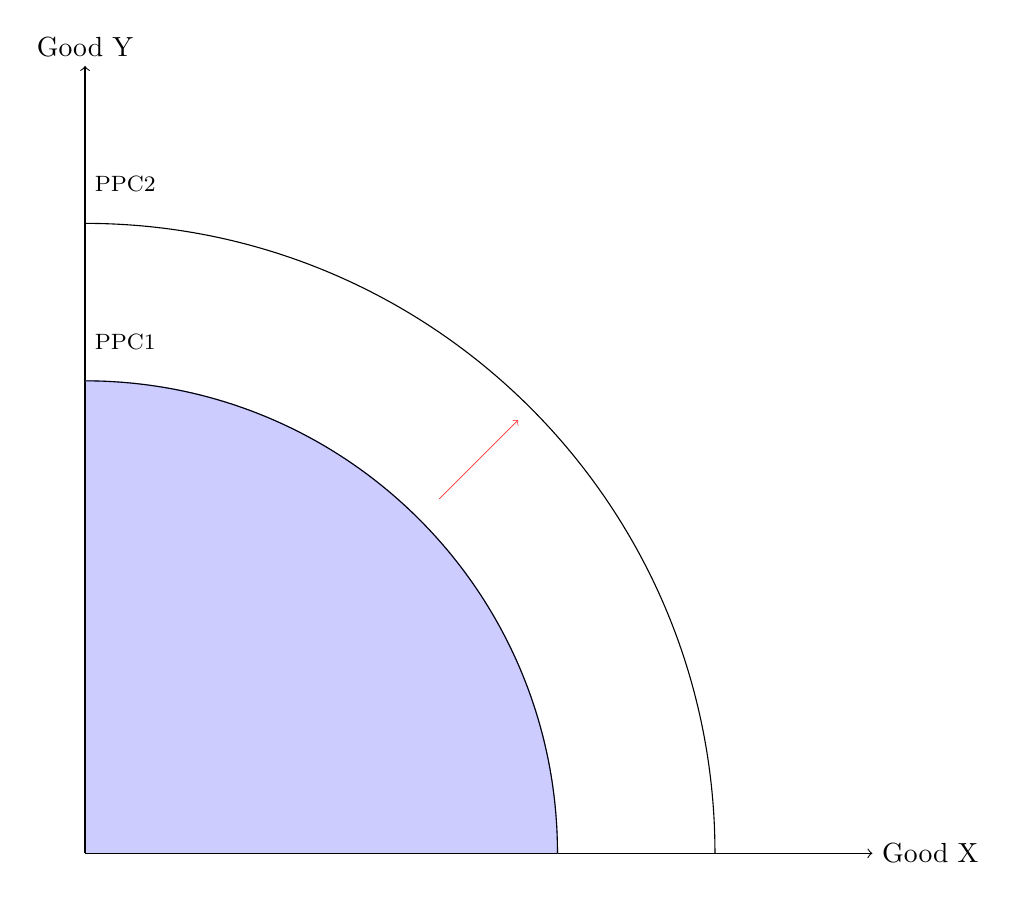
\begin{tikzpicture}
\fill[blue!20!white] (0,0)--(6,0) 
    arc [start angle=0, end angle=90, radius=6]--(0,0);
\draw[->](0,0)--(10,0) node[right]{Good X};
\draw[->](0,0)--(0,10) node[above]{Good Y};
\draw[thin,blue!40!white] (6,0) arc(0:90:6);
\draw[thin] (6,0) arc(0:90:6);
\draw[thin] (8,0) arc(0:90:8);
\draw[->,very thin,red] (4.5,4.5)--(5.5,5.5);
\draw (0,6.5)--(0,6.5) node[right] {\footnotesize PPC1};
\draw (0,8.5)--(0,8.5) node[right] {\footnotesize PPC2};
\end{tikzpicture}
\end{figure}
\\
\noindent
Every point inside the PPC or on the PPC is achievable by using partial resources or all resources (shaded area). Every point on the PPC is achieved by using all resources in one economy; Every point inside the PPC is achieved by using partial resources; Every point outside the PPC is not achievable.\\
\\
How to shift outward the PPC:\\
1. innovative technology\ \  2. more labors\ \  (an outward shift of PPC shows the economic growth)\\
\\
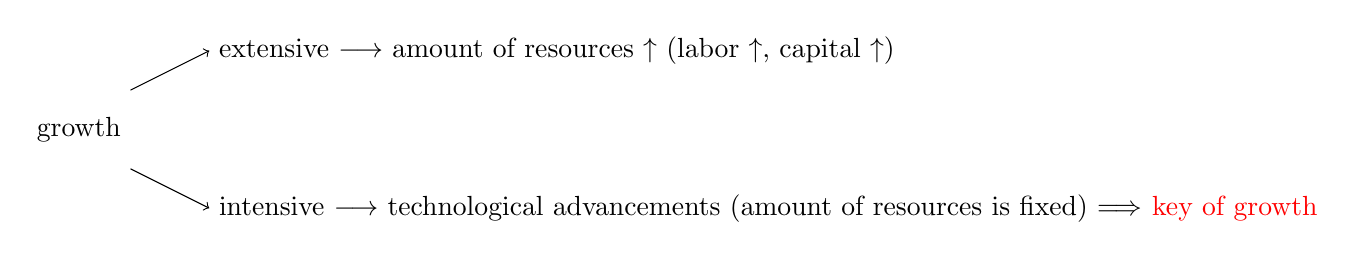
\begin{tikzpicture}
\draw (-0.5,3)--(-0.5,3) node[left]{growth};
\draw [->](-0.5,3.5)--(0.5,4);
\draw [->](-0.5,2.5)--(0.5,2);
\draw (0.5,4)--(0.5,4) node[right]{extensive $\longrightarrow$ amount of resources $\uparrow$ (labor $\uparrow$, capital $\uparrow$)};
\draw (0.5,2)--(0.5,2) node[right]{intensive $\longrightarrow$ technological advancements (amount of resources is fixed) $\Longrightarrow$};
\draw (12.35,2)--(12.35,2) node[right,red]{key of growth};
    
\end{tikzpicture}

\newpage
\subsection{Specialization in International Trade}
Both absolute advantage and comparative advantage are used to compare the production of a specific good in different economies. \\
\textbf{Absolute advantage}: which economy produce more in a given time \\
\textbf{Comparative advantage}: which economy produce with the lowest opportunity cost \\
* For the matrix of two economies and two goods, it's impossible for an economy to get two comparative advantages, but it's possible for an economy to get two absolute advantages.\\
\\
\\
\begin{table}[!h]
\centering
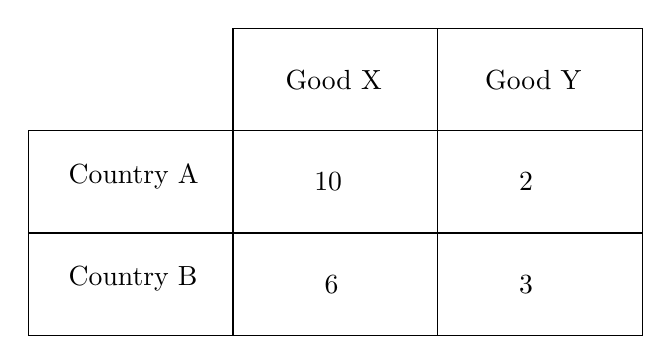
\begin{tikzpicture}[scale=1.3]
\draw (-2,0)--(-2,-2)--(4,-2)--(4,1)--(0,1)--(0,0)--(-2,0);
\draw (0,1)--(0,-2);
\draw (-2,0)--(4,0);
\draw (-2,0)--(-2,-2);
\draw (0,1)--(4,1);
\draw (-2,-1)--(4,-1);
\draw (2,1)--(2,-2);
\draw (-1.7,-0.45)--(-1.7,-0.45) node[right]{Country A};
\draw (1.55,0.5)--(1.55,0.5) node[left]{Good X};
\draw (-1.7,-1.45)--(-1.7,-1.45) node[right]{Country B};
\draw (3.5,0.5)--(3.5,0.5) node[left]{Good Y};
\draw (0.7,-0.5)--(0.7,-0.5) node[right]{10};
\draw (2.7,-0.5)--(2.7,-0.5) node[right]{2};
\draw (0.8,-1.5)--(0.8,-1.5) node[right]{6};
\draw (2.7,-1.5)--(2.7,-1.5) node[right]{3};
\end{tikzpicture}
\caption{example (production per hour)}
\end{table}

\noindent
How to analyze this example?\\
Apparently, Country A has absolute advantage on producing X (10 $>$ 6) and Country B has absolute advantage on producing Y (3 $>$ 2). For Country A, it has to give up $1\over 5$ unit of Y for producing X; for Country B, it has to give up $1\over 2$ unit of Y for producing X. $\Longrightarrow$ Country A has less opportunity cost on producing X $\Longrightarrow$ Country A has comparative advantage on producing X $\Longrightarrow$ Country B has comparative advantage on producing Y. So, Country A should produce X only and Country B should produce Y only, and the trade could happened between Country A and B.\\
Further, the possible price range for X = [ $1\over 5$Y, $1\over 2$Y ] (price between the possible price range will lead the trade to be happened)\\
$\rightarrow$ $1\over5$Y is the minimize selling price for Country A, and $1\over2$Y is the maximize buying price for Country B.\\

\newpage
\section{Demand and Supply}
\subsection{Demand}
\textbf{benefit} = value = how much you are willing to pay\\

\begin{table}[!h]
    \centering
    \begin{tabular}{|c|c|c|}
        \hline
        \# & Marginal Benefit & Total Benefit \\
        \hline
        1 & 10 & 10 \\
        \hline
        2 & 7 & 17 \\
        \hline
        3 & 4 & 21\\
        \hline
        4 & 2 & 23\\
        \hline
        5 & 0 & 23\\
        \hline
        6 & -10 & 13\\
        \hline
        7 & -13 & 0\\
        \hline
    \end{tabular}
    \caption{relationship between MB and TB}
    \label{tab:my_label}
\end{table}

\noindent
Consumer choice rule: if P $>$ MB $\rightarrow$ don't buy, if P $\le$ MB $\rightarrow$ buy\\
MB defined the maximum payment price (maximum willing to pay)\\
Determinants of willing to pay: $\mathcal{A}$: \textbf{utility} (satisfaction) $\mathcal{B}$: \textbf{wealth} (how much money or disposable income) $\mathcal{C}$: \textbf{other goods} (substitutions)\\

\noindent
\textbf{normal good}: Income$\uparrow$ $\Longrightarrow$ Demand$\uparrow$ \\
\textbf{inferior good}: Income$\uparrow$ $\Longrightarrow$ Demand$\downarrow$ \ \ \ \ \ \ \ \ \ e.g. instant noodles\\

\textbf{The law of demand:} P$\uparrow$ $\Longrightarrow$ Q$_D$$\downarrow$, P$\downarrow$ $\Longrightarrow$ Q$_D$$\uparrow$ (Downward sloping) \\
\begin{figure}[!h]
\begin{tikzpicture}
    \draw [->] (0,0)--(0,5);
    \draw (0,5)--(0,5) node[left]{P};
    \draw [->] (0,0)--(5,0);
    \draw (5,0)--(5,0) node[below]{Q$_D$};
    \draw (0.5,4)--(4.5,1) node[right]{D};
    \draw (6,3)--(6,3) node[right]{change in quantity demanded means points move along the demand curve};
    \draw (6,2.3)--(6,2.3) node[right]{change in demand means shifts of the demand curve};
\end{tikzpicture}
\end{figure}
\newpage
\noindent
\textbf{Demand shifters (Determinants)}:\\
\begin{figure}[!h]
\begin{tikzpicture}[scale=1.1]
    \draw [->] (0,0)--(0,5);
    \draw (0,5)--(0,5) node[left]{P};
    \draw [->] (0,0)--(5,0);
    \draw (5,0)--(5,0) node[below]{Q$_D$};
    \draw (0.5,4)--(4.5,1) node[right]{D$_1$};
    \draw (1,4.5)--(5,1.5) node[right]{D$_2$};
    \draw [->,color=red,thick] (2.2,3)--(2.7,3);
    \draw (2.5,-0.5)--(2.5,-0.5) node[below]{Demand curve shifts to the right (increase D $\uparrow$)};
    \draw [->] (8,0)--(8,5);
    \draw (8,5)--(8,5) node[left]{P};
    \draw [->] (8,0)--(13,0);
    \draw (13,0)--(13,0) node[below]{Q$_D$};
    \draw (8.5,4)--(12.5,1) node[right]{D$_1$};
    \draw (8,3.5)--(12,0.5) node[right]{D$_2$};
    \draw [<-,color=red,thick] (9,3)--(9.5,3);
    \draw (10.5,-0.5)--(10.5,-0.5) node[below]{Demand curve shifts to the left (decrease D $\downarrow$)};
\end{tikzpicture}
\end{figure}
\\
\textbf{1.} income $\uparrow$ $\Longrightarrow$ normal goods' D $\uparrow$ and inferior goods' D $\downarrow$\\
\textbf{2.} price of relative goods \textbf{(1)} P of substitutes $\uparrow$ $\Longrightarrow$ D $\uparrow$ \textbf{(2)} P of complements $\uparrow$ $\Longrightarrow$ D $\downarrow$\\
* \textbf{substitute}: for consumers, if they always choose $A$ rather than $B$ or $B$ rather than $A$, then $A$ and $B$ are substitute of each other. \ \ \ \ \ e.g. Pepsi \& Coca-Cola. \\
If there's a increase in price of Pepsi $\Longrightarrow$ there would be a decrease in quantity demanded of Pepsi $\Longrightarrow$ more people will choose Coca-Cola rather than Pepsi $\Longrightarrow$ there would be a increase in demand of Coca-Cola\\
* \textbf{complement}: for consumers, if they always choose $A$ and $B$ at the same time as a combination of consumption, then $A$ and $B$ are complement of each other. \ \ \ \ \ e.g. baseball \& baseball bat\\
If there's a increase in price of baseball bat $\Longrightarrow$ there would be a decrease in quantity demanded of baseball bat $\Longrightarrow$ less people will buy baseball bat and play baseball $\Longrightarrow$ there would also be a decrease in demand of baseball\\

\noindent
(\textbf{1.} and \textbf{2.} are keys in the AP exam)\\
3. expectation\\
4. utility\\
5. number of buyers\\

\newpage
\subsection{Supply}
\begin{figure}[!h]
\begin{tikzpicture}
    \draw [->] (0,0)--(0,5);
    \draw (0,5)--(0,5) node[left]{P};
    \draw [->] (0,0)--(5,0);
    \draw (5,0)--(5,0) node[below]{Q$_S$};
    \draw (0.5,1)--(4.5,4) node[right]{S};
    \draw (6,3)--(6,3) node[right]{\textbf{The law of supply}: P$\uparrow$ $\Longrightarrow$ Q$_S$$\uparrow$, P$\downarrow$ $\Longrightarrow$ Q$_S$$\downarrow$ (Upward sloping) };
    \draw (6,2.2)--(6,2.2) node[right]{S = marginal cost = minimized selling price};
\end{tikzpicture}
\end{figure}
\textbf{Supply shifters (Determinants)}:\\
\begin{figure}[!h]
\begin{tikzpicture}[scale=1.1]
    \draw [->] (0,0)--(0,5);
    \draw (0,5)--(0,5) node[left]{P};
    \draw [->] (0,0)--(5,0);
    \draw (5,0)--(5,0) node[below]{Q$_S$};
    \draw (0.5,1)--(4.5,4) node[right]{S$_1$};
    \draw (1,0.5)--(5,3.5) node[right]{S$_2$};
    \draw [->,color=red,thick] (3.4,3)--(3.9,3);
    \draw (2.5,-0.5)--(2.5,-0.5) node[below]{Supply curve shifts to the right (increase S $\uparrow$)};
    \draw [->] (8,0)--(8,5);
    \draw (8,5)--(8,5) node[left]{P};
    \draw [->] (8,0)--(13,0);
    \draw (13,0)--(13,0) node[below]{Q$_S$};
    \draw (8.5,1)--(12.5,4) node[right]{S$_1$};
    \draw (8,1.5)--(12,4.5) node[right]{S$_2$};
    \draw [<-,color=red,thick] (10.3,3)--(10.8,3);
    \draw (10.5,-0.5)--(10.5,-0.5) node[below]{Supply curve shifts to the left (decrease S $\downarrow$)};
\end{tikzpicture}
\end{figure}
\\
\textbf{1. } input cost $\uparrow$ (price of raw material $\uparrow$ or wage $\uparrow$) $\Longrightarrow$ S $\downarrow$\\
\textbf{2. } productive substitutes or complements \\
\textbf{3. } technology\\
\noindent
4. \ \ expectation\\
5. \ \  number of seller \\

\newpage
\subsection{Market Equilibrium}
\begin{figure}[h!]
\begin{tikzpicture}[scale=0.8]
\draw [->] (0,0)--(0,10);
\draw (0,10)--(0,10) node[left]{P};
\draw [->] (0,0)--(10,0);
\draw (10,0)--(10,0) node[below]{Q};
\draw (0.5,0.3)--(8.8,8) node[right]{S};
\draw (0.5,8)--(8.8,0.3) node[right]{D};
\draw[dotted] (4.65,4.15)--(4.65,0) node[below]{Q$_e$};
\draw[dotted] (4.65,4.15)--(0,4.15) node[left]{P$_e$};
\node[circle,fill=black,inner sep = 1.2pt] (A1) at (4.65,4.15) {};
\draw (4.8,4.15)--(4.8,4.15) node[right]{$\longrightarrow$ \ \ equilibrium point};
\end{tikzpicture}
\end{figure}
\subsection{Efficiency}
\begin{definition}
maximum wealth measured in value
\end{definition}
surplus(consumer surplus and producer surplus) $\Longrightarrow$ difference between the value and the price\\

\begin{figure}[h]
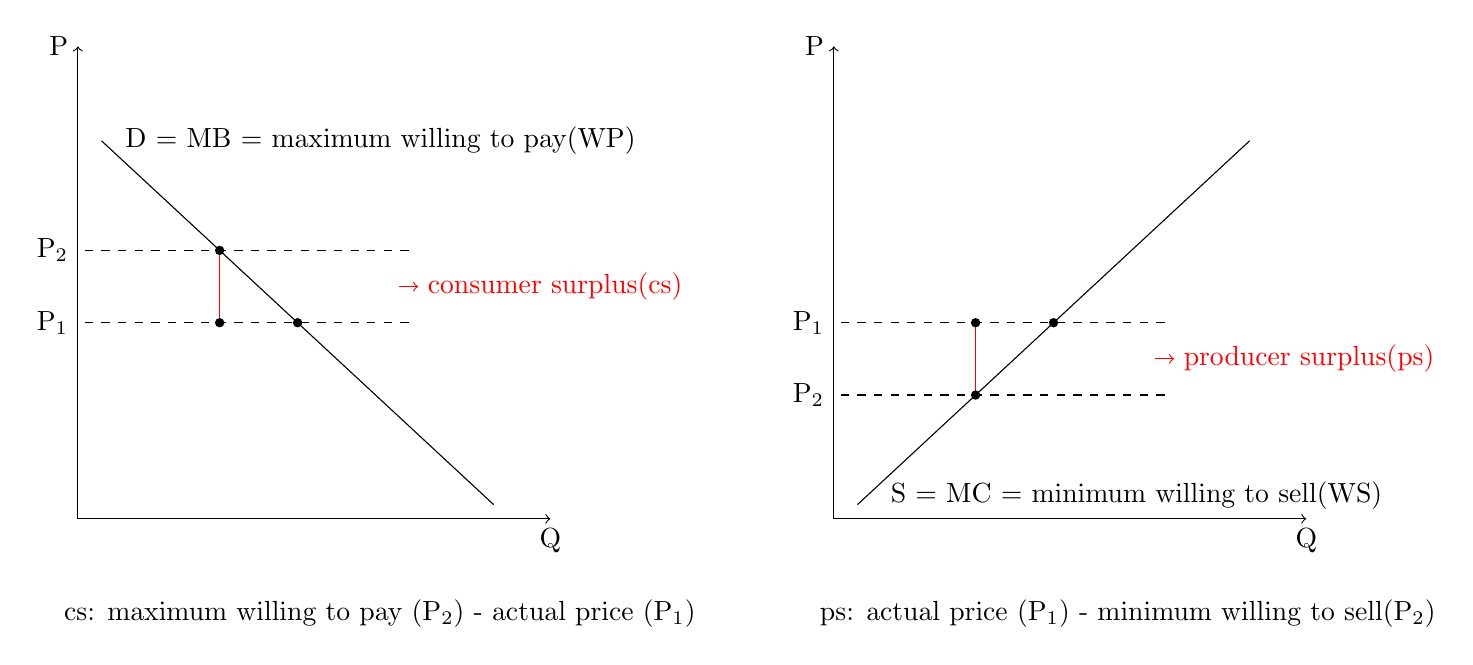
\begin{tikzpicture}[scale=0.6]
\draw [->] (0,0)--(0,10);
\draw (0,10)--(0,10) node[left]{P};
\draw[red](3,5.680722892)--(3,4.15);
\draw [->] (0,0)--(10,0);
\draw (10,0)--(10,0) node[below]{Q};   
\draw (8.8,0.3)--(0.5,8);
\draw (0.8,8)--(0.8,8)node[right]{D = MB = maximum willing to pay(WP)};
\draw[dashed] (7,4.15)--(0,4.15) node[left]{P$_1$};
\node[circle,fill=black,inner sep = 1.2pt] (A1) at (4.65,4.15) {};
\node[circle,fill=black,inner sep = 1.2pt] (A2) at (3,5.680722892) {};
\node[circle,fill=black,inner sep = 1.2pt] (A3) at (3,4.15) {};
\draw[dashed] (7,5.680722892)--(0,5.680722892) node[left]{P$_2$};
\draw[->,red](6.8,4.915)--(7.2,4.915) node[right]{consumer surplus(cs)};
\draw (-0.5,-2)--(-0.5,-2) node[right]{cs: maximum willing to pay (P$_2$) - actual price (P$_1$)};

\draw [->] (16,0)--(16,10);
\draw (16,10)--(16,10) node[left]{P};
\draw [->] (16,0)--(26,0);
\draw (26,0)--(26,0) node[below]{Q};   
\draw (24.8,8)--(16.5,0.3);
\draw (17,0.5)--(17,0.5)node[right]{S = MC = minimum willing to sell(WS)};
\draw[red](19,2.619277108)--(19,4.15);
\draw[dashed] (23,4.15)--(16,4.15) node[left]{P$_1$};
\node[circle,fill=black,inner sep = 1.2pt] (A1) at (20.65,4.15) {};
\draw[->,red](22.8,3.385)--(23.2,3.385) node[right]{producer surplus(ps)};
\node[circle,fill=black,inner sep = 1.2pt] (A2) at (19,2.619277108) {};
\node[circle,fill=black,inner sep = 1.2pt] (A3) at (19,4.15) {};
\draw[dashed](23,2.619277108)--(16,2.619277108) node[left]{P$_2$};
\draw (15.5,-2)--(15.5,-2) node[right]{ps: actual price (P$_1$) - minimum willing to sell(P$_2$)};
\end{tikzpicture}
\end{figure}

\newpage
\noindent
Total surplus (TS) = CS + PS = WP-WS = MB-MC\\
* The product will flow from the low value to the high value\\
\textbf{Allocative efficiency}: occurs when the total surplus is maximized. \\
$\because$ TS = TB $-$ TC (the following steps are based on derivative)\\
$\therefore$ TS$_{max}$ occurs when TS$'$ = 0 $\rightarrow$ TB$'$ $-$ TC$'$ = 0 $\rightarrow$ MB $-$ MC = 0\\
$\therefore$ when MB = MC, the $\Sigma$TS will be maximized.\\
\begin{figure}[h!]
\begin{center}
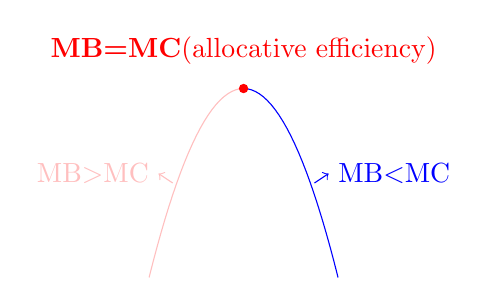
\begin{tikzpicture}[scale=0.6]
\draw[pink,domain=-2:0] plot(\x,-\x*\x);
\draw[blue,domain=0:2] plot(\x,-\x*\x);
\node[circle,fill=red,inner sep = 1.2pt] (A1) at (0,0) {};
\draw [red](0,0.3)--(0,0.3) node[above]{\textbf{MB=MC}(allocative efficiency)};
\draw[pink,->](-1.5,-2)--(-1.8,-1.8) node[left]{MB$>$MC};
\draw[blue,->](1.5,-2)--(1.8,-1.8) node[right]{MB$<$MC};
\end{tikzpicture}
\caption{The level of this curve represent the value of total surplus.\\
*\textbf{When MB$>$MC, Q$\uparrow$ $\longrightarrow$ $\Sigma$TS$\uparrow$; when MB$<$MC, Q$\uparrow$ $\longrightarrow$ $\Sigma$TS$\downarrow$.}}
\end{center}
\end{figure}
\subsection{Dead Weight Loss (DWL)}
\textbf{DWL = maximized potential total surplus $-$ current total surplus}\\
Two type of DWL: (1) under allocation: the quantity traded is under the equilibrium quantity. \\
(2) over allocation: the quantity traded is over the equilibrium quantity.\\
* By noticing the TS and DWL, when DWL occurs, the TS is not at the maximum.\\
\begin{figure}[h!]
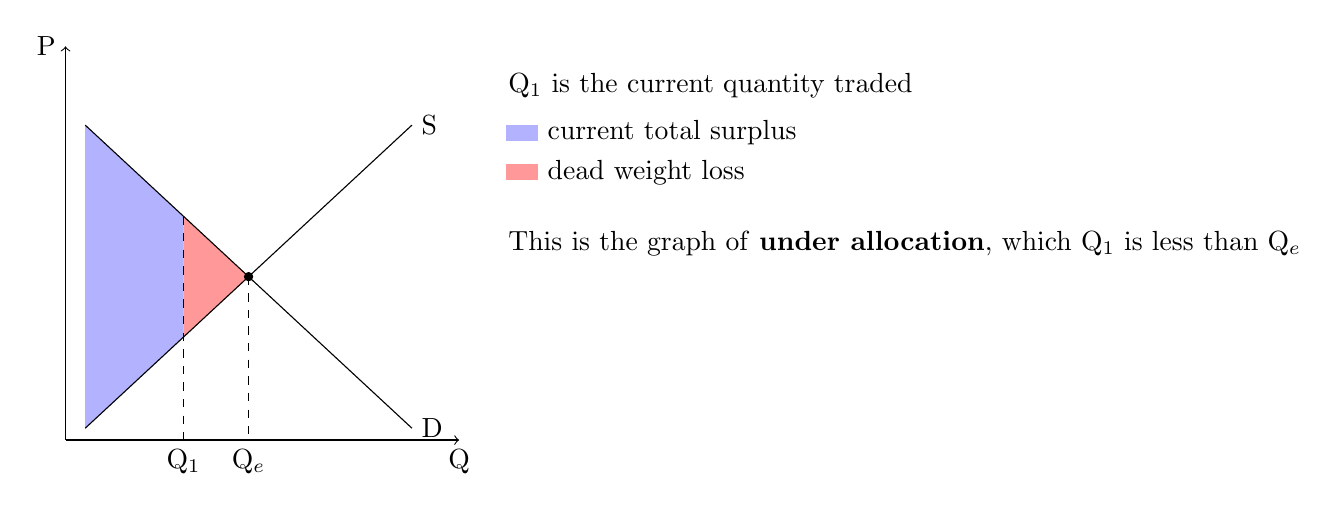
\begin{tikzpicture}[scale=0.5]
\fill[blue!30!white] (0.5,0.3)--(0.5,8)--(3,5.680722892)--(3,2.619277108);
\fill[red!40!white] (3,5.680722892)--(3,2.619277108)--(4.65,4.15);
\draw [->] (0,0)--(0,10);
\draw (0,10)--(0,10) node[left]{P};
\draw [->] (0,0)--(10,0);
\draw (10,0)--(10,0) node[below]{Q};
\draw (0.5,0.3)--(8.8,8) node[right]{S};
\draw (0.5,8)--(8.8,0.3) node[right]{D};
\draw[dashed] (4.65,4.15)--(4.65,0) node[below]{Q$_e$};
\node[circle,fill=black,inner sep = 1.2pt] (A1) at (4.65,4.15) {};
\draw[dashed](3,5.680722892)--(3,0) node[below]{Q$_1$};
\draw (11,9)--(11,9) node[right]{Q$_1$ is the current quantity traded};
\fill[blue!30!white] (11.2,8)--(12,8)--(12,7.6)--(11.2,7.6);
\draw (12,7.8)--(12,7.8) node[right]{current total surplus};
\fill[red!40!white](11.2,7)--(12,7)--(12,6.6)--(11.2,6.6);
\draw (12,6.8)--(12,6.8) node[right]{dead weight loss};
\draw (11,5)--(11,5) node[right]{This is the graph of \textbf{under allocation}, which Q$_1$ is less than Q$_e$};
\end{tikzpicture}
\end{figure}

\newpage
\subsection{Taxation}
\noindent
\begin{definition}
Taxation: governments uses its power to collect money or resources from people. 
\end{definition}

\textbf{different types of tax: }

1. sales tax (on consumer)/ excise tax (on producer)

2. lump-sum tax $\rightarrow$ fixed amount of tax

3. income tax\\
\\

*Government Revenue (tax): per unit tax$\times Q_{tax}$


\begin{figure}[!h]
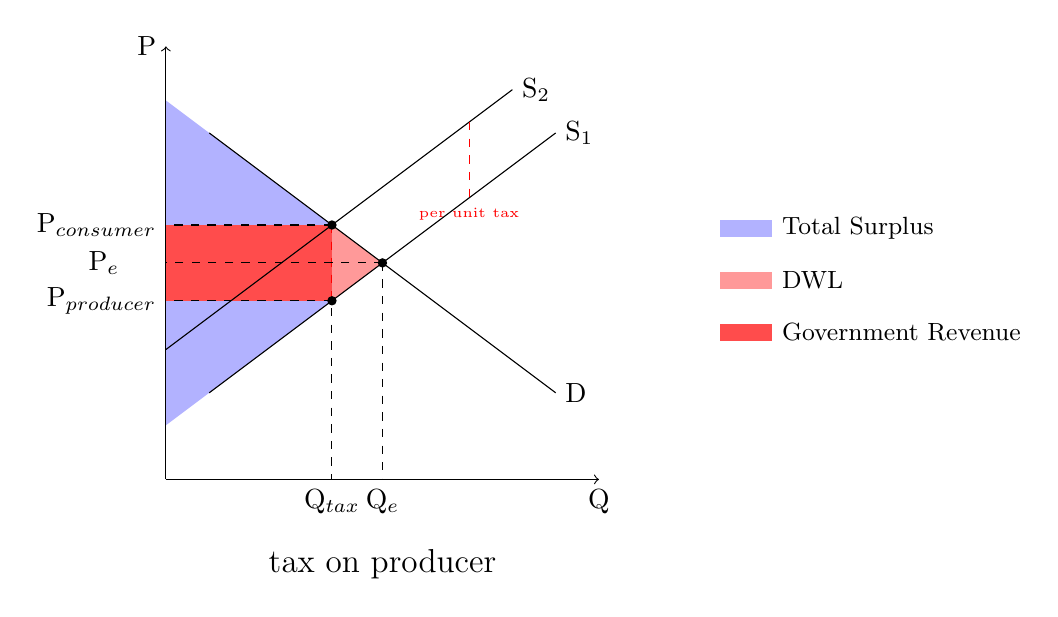
\begin{tikzpicture}[scale=1.1]
    \fill[red!40!white] (2.5,2.5)--(1.9167,2.9375)--(1.9167,2.0625);
    \fill[blue!30!white] (1.9167,2.0625)--(0,0.625)--(0,2.0625);
    \fill[blue!30!white] (1.9167,2.9375)--(0,2.9375)--(0,4.375);
    \fill[red!70!white] (1.9167,2.0625)--(1.9167,2.9375)--(0,2.9375)--(0,2.0625);
    \draw [->] (0,0)--(0,5);
    \draw (0,5)--(0,5) node[left]{P};
    \draw [->] (0,0)--(5,0);
    \draw (5,0)--(5,0) node[below]{Q};
    \draw (0.5,1)--(4.5,4) node[right]{S$_1$};
    \draw (0,1.5)--(4,4.5) node[right]{S$_2$};
    \draw (0.5,4)--(4.5,1) node[right]{D};
    \draw (2.5,-0.7)--(2.5,-0.7) node[below]{\large tax on producer};
    \draw[dashed] (2.5,2.5)--(2.5,0) node[below]{Q$_e$};
    \draw[dashed] (1.9167,2.9375)--(1.9167,0) node[below]{Q$_{tax}$};
    \draw[dashed,red] (1.9167,2.9375)--(1.9167,2.0625);
    \draw[dashed,red] (3.5,4.125)--(3.5,3.25) node[below]{\tiny per unit tax};
    \node[circle,fill=black,inner sep = 1.2pt] (A1) at (2.5,2.5) {};
    \node[circle,fill=black,inner sep = 1.2pt] (A1) at (1.9167,2.9375) {};
    \node[circle,fill=black,inner sep = 1.2pt] (A1) at (1.9167,2.0625) {};
    \draw[dashed] (1.9167,2.9375)--(0,2.9375) node[left]{P$_{consumer}$};
    \draw[dashed] (1.9167,2.0625)--(0,2.0625) node[left]{P$_{producer}$};
    \draw[dashed] (2.5,2.5)--(0,2.5) node[left]{P$_e$\ \ \ \ \ };
    \fill[blue!30!white] (6.4,3)--(7,3)--(7,2.8)--(6.4,2.8);
    \fill[red!40!white](6.4,2.4)--(7,2.4)--(7,2.2)--(6.4,2.2);
    \fill[red!70!white](6.4,1.8)--(7,1.8)--(7,1.6)--(6.4,1.6);
    \draw (7,2.9)--(7,2.9) node[right]{\small Total Surplus};
    \draw (7,2.3)--(7,2.3) node[right]{\small DWL};
    \draw (7,1.7)--(7,1.7) node[right]{\small Government Revenue};
\end{tikzpicture}
\end{figure}


\begin{figure}[!h]
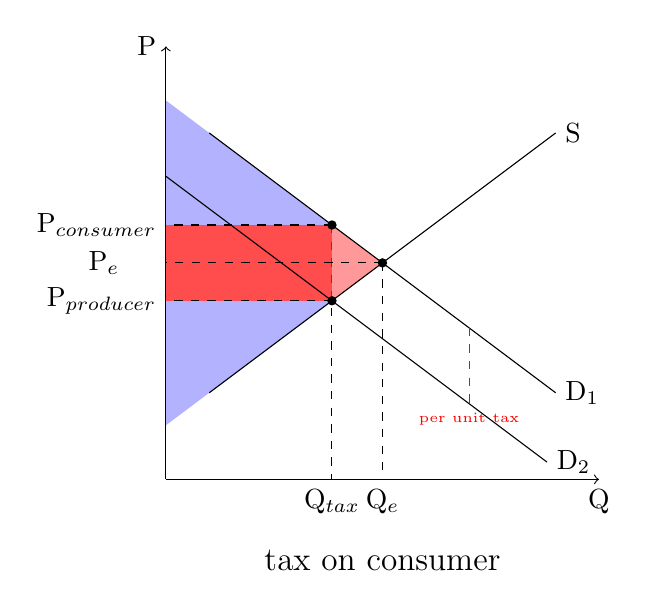
\begin{tikzpicture}[scale=1.1]
    \fill[red!40!white] (2.5,2.5)--(1.9167,2.9375)--(1.9167,2.0625);
    \fill[blue!30!white] (1.9167,2.0625)--(0,0.625)--(0,2.0625);
    \fill[blue!30!white] (1.9167,2.9375)--(0,2.9375)--(0,4.375);
    \fill[red!70!white] (1.9167,2.0625)--(1.9167,2.9375)--(0,2.9375)--(0,2.0625);
    \draw [->] (0,0)--(0,5);
    \draw (0,5)--(0,5) node[left]{P};
    \draw [->] (0,0)--(5,0);
    \draw (5,0)--(5,0) node[below]{Q};
    \draw (0.5,1)--(4.5,4) node[right]{S};
    \draw (0.5,4)--(4.5,1) node[right]{D$_1$};
    \draw (0,3.5)--(4.4,0.2) node[right]{D$_2$};
    \draw (2.5,-0.7)--(2.5,-0.7) node[below]{\large tax on consumer};
    \draw[dashed] (2.5,2.5)--(2.5,0) node[below]{Q$_e$};
    \draw[dashed] (1.9167,2.9375)--(1.9167,0) node[below]{Q$_{tax}$};
    \draw[dashed,red] (1.9167,2.9375)--(1.9167,2.0625);
    \draw[dashed,red] (3.5,1.75 )--(3.5,0.875) node[below]{\tiny per unit tax};
    \node[circle,fill=black,inner sep = 1.2pt] (A1) at (2.5,2.5) {};
    \node[circle,fill=black,inner sep = 1.2pt] (A1) at (1.9167,2.9375) {};
    \node[circle,fill=black,inner sep = 1.2pt] (A1) at (1.9167,2.0625) {};
    \draw[dashed] (1.9167,2.9375)--(0,2.9375) node[left]{P$_{consumer}$};
    \draw[dashed] (1.9167,2.0625)--(0,2.0625) node[left]{P$_{producer}$};
    \draw[dashed] (2.5,2.5)--(0,2.5) node[left]{P$_e$\ \ \ \ \ };
\end{tikzpicture}
\end{figure}

Result: tax prevents the potential trades to happen (create DWL)

If tax is greater than the TS, the trade would not happen.

\begin{tabular}{c|c|c}
    value & if tax: 1095 & if tax: 1095 \\
    \hline
    A: 10 (sell) & B: 5 to buy at most & A: 1105 to sell at least \\
    B: 1100 (buy) & 5<10, no trade & 1105>1100, no trade\\
    
\end{tabular}
\\
\subsection{Subsidy}
* Subsidy is a sort of reverse of tax.
\begin{figure}[!h]
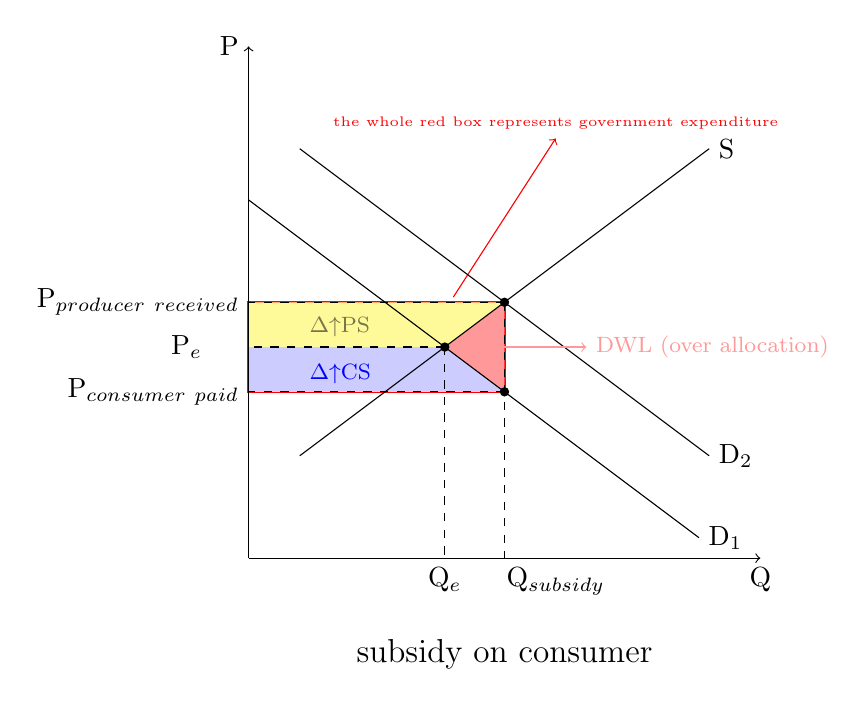
\begin{tikzpicture}[scale=1.3]
    \draw[red,very thick] (2.5,2.5)--(2.5,1.625)--(0,1.625)--(0,2.5)--(2.5,2.5);
    \draw[->,red,thin] (2,2.55)--(3,4.1) node[above]{\tiny the whole red box represents government expenditure};
    \fill[red!40!white] (2.5,2.5)--(1.9167,2.0625)--(2.5,1.625);
    \fill[blue!20!white] (1.9167,2.0625)--(2.5,1.625)--(0,1.625)--(0,2.0625);
    \draw (0.5,1.8)--(0.5,1.8) node[right,blue]{\footnotesize $\Delta$$\uparrow$CS};
    \fill[yellow!40!white] (1.9167,2.0625)--(2.5,2.5)--(0,2.5)--(0,2.0625);
    \draw (0.5,2.26)--(0.5,2.26) node[right,yellow!40!black]{\footnotesize $\Delta$$\uparrow$PS};
    \draw [->] (0,0)--(0,5);
    \draw (0,5)--(0,5) node[left]{P};
    \draw [->] (0,0)--(5,0);
    \draw (5,0)--(5,0) node[below]{Q};
    \draw (0.5,1)--(4.5,4) node[right]{S};
    \draw (0.5,4)--(4.5,1) node[right]{D$_2$};
    \draw (0,3.5)--(4.4,0.2) node[right]{D$_1$};
    \draw (2.5,-0.7)--(2.5,-0.7) node[below]{\large subsidy on consumer};
    \node[circle,fill=black,inner sep = 1.2pt] (A1) at (1.9167,2.0625) {};
    \draw[dashed] (1.9167,2.0625)--(1.9167,0) node[below]{Q$_e$};
    \node[circle,fill=black,inner sep = 1.2pt] (A1) at (2.5,2.5) {};
    \draw[dashed] (2.5,2.5)--(2.5,0);
    \draw (3,0)--(3,0) node[below]{Q$_{subsidy}$};
    \node[circle,fill=black,inner sep = 1.2pt] (A1) at (2.5,1.625) {};
    \draw[dashed] (2.5,1.625)--(0,1.625) node[left]{P$_{consumer\ paid}$};
    \draw[dashed] (2.5,2.5)--(0,2.5) node[left]{P$_{producer\ received}$};
    \draw[dashed] (1.9167,2.0625)--(0,2.0625) node[left]{P$_e$\ \ \ \ \ };
    \draw[->,red!40!white] (2.4,2.0625)--(3.3,2.0625) node[right,red!40!white]{\footnotesize DWL (over allocation)};

\end{tikzpicture}
\end{figure}
\subsection{Price Control}

\begin{figure}[!h]
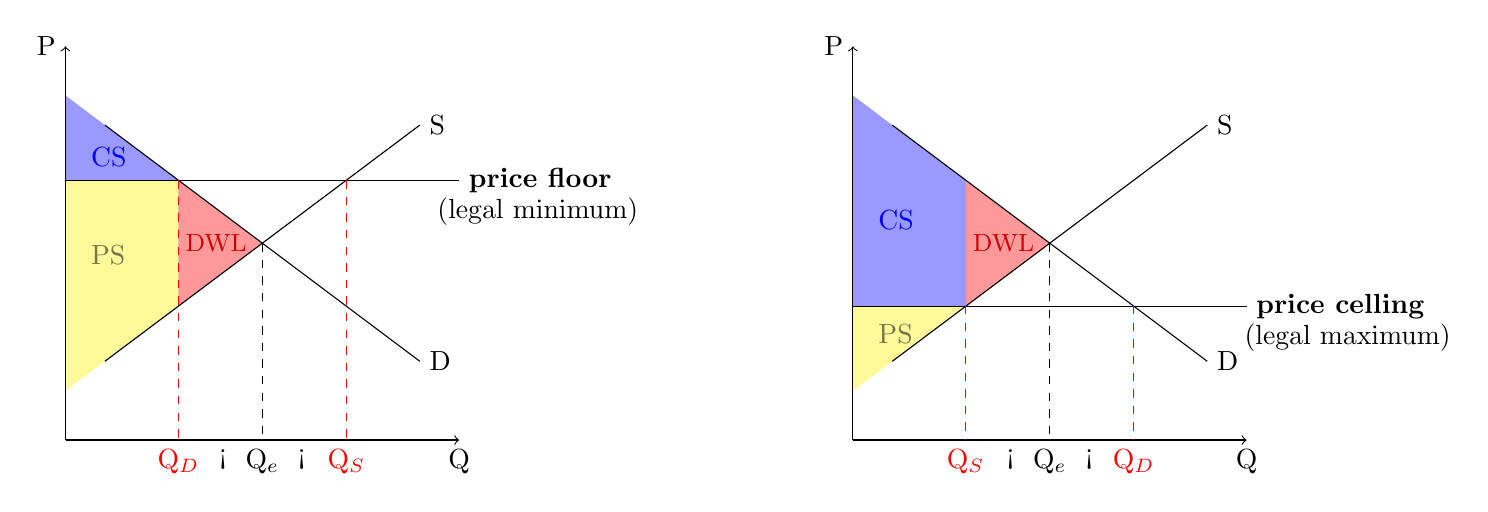
\begin{tikzpicture}
    \fill[blue!40!white] (1.433,3.3)--(0,3.3)--(0,4.375);
    \fill[yellow!40!white] (1.433,3.3)--(0,3.3)--(0,0.625)--(1.433,1.7);
    \fill[red!40!white] (1.433,3.3)--(2.5,2.5)--(1.433,1.7);
    \draw [->] (0,0)--(0,5);
    \draw (0,5)--(0,5) node[left]{P};
    \draw [->] (0,0)--(5,0);
    \draw (5,0)--(5,0) node[below]{Q};
    \draw (0.5,1)--(4.5,4) node[right]{S};
    \draw (0.5,4)--(4.5,1) node[right]{D};
    \draw (0,3.3)--(5,3.3) node[right]{\textbf{price floor}};
    \draw (4.6,2.9)--(4.6,2.9) node[right]{(legal minimum)};
    \draw (1.4,2.5)--(1.4,2.5) node[right,red!80!black]{\small DWL};
    \draw[dashed,red] (1.433,3.3)--(1.433,0) node[below]{Q$_D$};
    \draw[dashed,red] (3.567,3.3)--(3.567,0) node[below]{Q$_S$};
    \draw[dashed] (2.5,2.5)--(2.5,0) node[below]{Q$_e$};
    \draw (2,0)--(2,0) node[below]{<};
    \draw (3,0)--(3,0) node[below]{<};
    \draw (0.2,3.6)--(0.2,3.6) node[right,blue]{CS};
    \draw (0.2,2.35)--(0.2,2.35) node[right,yellow!40!black]{PS};

    \fill[blue!40!white] (11.433,1.7)--(11.433,3.3)--(10,4.375)--(10,1.7);
    \fill[yellow!40!white] (10,1.7)--(11.433,1.7)--(10,0.625);
    \fill[red!40!white] (11.433,3.3)--(12.5,2.5)--(11.433,1.7);
    \draw [->] (10,0)--(10,5);
    \draw (10,5)--(10,5) node[left]{P};
    \draw [->] (10,0)--(15,0);
    \draw (15,0)--(15,0) node[below]{Q};
    \draw (10.5,1)--(14.5,4) node[right]{S};
    \draw (10.5,4)--(14.5,1) node[right]{D};
    \draw (10,1.7)--(15,1.7) node[right]{\textbf{price celling}};
    \draw (14.85,1.3)--(14.85,1.3) node[right]{(legal maximum)};
    \draw (11.4,2.5)--(11.4,2.5) node[right,red!80!black]{\small DWL};
    \draw[dashed,red] (11.433,1.7)--(11.433,0) node[below]{Q$_S$};
    \draw[dashed,red] (13.567,1.7)--(13.567,0) node[below]{Q$_D$};
    \draw[dashed] (12.5,2.5)--(12.5,0) node[below]{Q$_e$};
    \draw (12,0)--(12,0) node[below]{<};
    \draw (13,0)--(13,0) node[below]{<};
    \draw (10.2,2.8)--(10.2,2.8) node[right,blue]{CS};
    \draw (10.2,1.35)--(10.2,1.35) node[right,yellow!40!black]{PS};
\end{tikzpicture}  
\end{figure}
\newpage
\subsection{Elasticity}
\noindent
\textbf{price elasticity of demand (PED):}

\textbf{1. price inelastic:} buyer are not highly responsive to the change in price (lack of substitute goods).

P changes $\longrightarrow$ small change in Q$_D$ $\longrightarrow$ price inelastic (e.g. rice, water)

\textbf{2. price elastic:} buyer are highly responsive to the change in price (some substitute goods)

P changes $\longrightarrow$ large change in Q$_D$ $\longrightarrow$ price elastic (e.g. coca cola)

\begin{equation}
    \text{price elasticity of demand (PED)} = {{\% \Delta \text{Q}_D}\over \% \Delta \text{P}}
    \nonumber
\end{equation}

* if the |PED|<1 $\Longrightarrow$ price inelastic ( $\because$ \%$\Delta$Q$_D$<\%$\Delta$P)

* if the |PED|>1 $\Longrightarrow$ price elastic ( $\because$ \%$\Delta$Q$_D$>\%$\Delta$P)

\begin{figure}[!h]
\begin{tikzpicture}[scale=1.2]
    \draw [->] (0,0)--(0,5);
    \draw (0,5)--(0,5) node[left]{P};
    \draw [->] (0,0)--(5,0);
    \draw (5,0)--(5,0) node[below]{Q};
    \draw (2.5,-0.37)--(2.5,-0.37) node[below]{\large inelastic demand curve};
    \draw (0.5,4)--(2.5,0.5) node[right]{\large D};
    \draw[dashed] (0.5,4)--(4,4);
    \draw[dashed,red,thick] (0.5,4)--(0.5,0.5);
    \draw[dashed,red,thick] (0.5,4)--(4,0.5);
    \node[circle,fill=black,inner sep = 1.2pt] (A1) at (1.2,2.775) {};
    \node[circle,fill=black,inner sep = 1.2pt] (A1) at (1.8,1.725) {};
    \draw[dotted,thin] (1.2,2.775)--(0,2.775) node[left]{P};
    \draw[dotted,thin] (1.2,2.775)--(1.2,0) node[below]{Q};
    \draw[dotted,thin] (1.8,1.725)--(0,1.725) node[left]{P'};
    \draw[dotted,thin] (1.8,1.725)--(1.8,0) node[below]{Q'};
    \draw[red,->,thick] (0,2.775)--(0,1.725);
    \draw[red,->,thick] (0,1.725)--(0,2.775);
    \draw[red,->,thick] (1.8,0)--(1.2,0);
    \draw[red,->,thick] (1.2,0)--(1.8,0);











    \draw [->] (7,0)--(7,5);
    \draw (7,5)--(7,5) node[left]{P};
    \draw [->] (7,0)--(12,0);
    \draw (12,0)--(12,0) node[below]{Q};
    \draw (9.5,-0.37)--(9.5,-0.37) node[below]{\large elastic demand curve};
    \draw (7.5,4)--(11.5,2) node[right]{\large D};
    \draw[dashed,red,thick] (7.5,4)--(11,4);
    \draw[dashed] (7.5,4)--(7.5,0.5);
    \draw[dashed,red,thick] (7.5,4)--(11,0.5);
    \node[circle,fill=black,inner sep = 1.2pt] (A1) at (9,3.25) {};
    \node[circle,fill=black,inner sep = 1.2pt] (A1) at (10.5,2.5) {};
    \draw[dotted,thin] (9,3.25)--(7,3.25) node[left]{P};
    \draw[dotted,thin] (9,3.25)--(9,0) node[below]{Q};
    \draw[dotted,thin] (10.5,2.5)--(7,2.5) node[left]{P'};
    \draw[dotted,thin] (10.5,2.5)--(10.5,0) node[below]{Q'};
    \draw[red,->,thick] (7,3.25)--(7,2.5);
    \draw[red,->,thick] (7,2.5)--(7,3.25);
    \draw[red,->,thick] (9,0)--(10.5,0);
    \draw[red,->,thick] (10.5,0)--(9,0);
    
\end{tikzpicture}
\end{figure}


when |PED|=0 $\Longrightarrow$ demand is perfectly price inelastic $\Longrightarrow$ $\Delta$P will not affect Q$_D$ ( $\because$ no substitute)

when |PED|=$+\infty$ $\Longrightarrow$ demand is perfectly price elastic $\Longrightarrow$ $\Delta$P $\rightarrow$ Q$_D$=0 ( $\because$ many substitutes)

when |PED|=1 $\Longrightarrow$ unitary price elasticity $\Longrightarrow$ \%$\Delta$Q$_D$ is proportional to \%$\Delta$P

\begin{figure}[!h]
\begin{tikzpicture}[scale=1.1]
    \draw [->] (0,0)--(0,3);
    \draw (0,3)--(0,3) node[left]{P};
    \draw [->] (0,0)--(3,0);
    \draw (3,0)--(3,0) node[below]{Q};
    \draw (7.5,0)--(7.5,2.5) node[right]{D};
    \draw (7.5,-0.1)--(7.5,-0.1) node[below]{|PED|=0};


    \draw [->] (6,0)--(6,3);
    \draw (6,3)--(6,3) node[left]{P};
    \draw [->] (6,0)--(9,0);
    \draw (9,0)--(9,0) node[below]{Q};
    \draw (12,1.5)--(14.5,1.5) node[right]{D};
    \draw (13.5,-0.1)--(13.5,-0.1) node[below]{|PED|=$+\infty$};


    \draw [->] (12,0)--(12,3);
    \draw (12,3)--(12,3) node[left]{P};
    \draw [->] (12,0)--(15,0);
    \draw (15,0)--(15,0) node[below]{Q};
    \begin{axis}[
    axis lines=none,
    xmin=0, xmax=3,
    ymin=0, ymax=3,
    samples=200,
    domain=0.15:1.2
    ]
    \addplot[thick] {0.2/x};
    \end{axis}
    \draw (1.5,-0.1)--(1.5,-0.1) node[below]{|PED|=1};
\end{tikzpicture}
\end{figure}

\newpage

Substitutions:

substitutions $\uparrow$ $\Longrightarrow$ PED $\uparrow$ (easy to be replaced), substitutions $\downarrow$ $\Longrightarrow$ PED $\downarrow$ (hard to be replaced)\\

Relationship between PED \& revenue ( $\because$ revenue = P$\times$Q):\\
\begin{tabular}{|c|c|c|c|}
    \hline
    price change & inelastic demand & unitary demand & elastic demand\\
    \hline
    price $\Uparrow$ & revenue $\Uparrow$ & no change & revenue $\Downarrow$\\
    \hline
    price $\Downarrow$ & revenue $\Downarrow$ & no change & revenue $\Uparrow$\\
    \hline
    
\end{tabular}\\
\\
$\longrightarrow$ price discrimination: occurs when firms charge different consumers different prices for the same product due to differences in PED.
\\
\\
\textbf{Midpoint Elasticity:}
\begin{figure}[!h]
\begin{tikzpicture}
    \draw [->] (0,0)--(0,5);
    \draw (0,5)--(0,5) node[left]{P};
    \draw [->] (0,0)--(5,0);
    \draw (5,0)--(5,0) node[below]{Q};
    \draw[thick](0.3,4.5)--(4.5,0.5) node[right]{D};
    \node[circle,fill=black,inner sep = 1.8pt] (A1) at (1.5,3.357) {};
    \node[circle,fill=black,inner sep = 1.8pt] (A1) at (3.5,1.452) {};
    \draw (1.5,3.357)--(1.5,3.357) node[right]{\ \ A (P$_1$,Q$_1$)};
    \draw (3.5,1.452)--(3.5,1.452) node[right]{\ \ B (P$_2$,Q$_2$)};
    \draw (8,2.7)--(8,2.7) node[right]{\Large $\epsilon$\ = $\%\Delta \text{Q}\over \%\Delta \text{P}$ = };
    \draw (11,2.7)--(14,2.7);
    \draw (12.5,2.7)--(12.5,2.7) node[above]{2};
    \draw (12.5,2.7)--(12.5,2.7) node[below]{$\text{P}_2-\text{P}_1$};
    \draw (11.8,3.2)--(13.2,3.2);
    \draw (12.5,3.2)--(12.5,3.2) node[above]{$\text{Q}_1+\text{Q}_2$};
    \draw (11.4,3.8)--(13.6,3.8);
    \draw (12.5,3.8)--(12.5,3.8) node[above]{$\text{Q}_2-\text{Q}_1$};
    \draw (11.4,2.2)--(13.6,2.2);
    \draw (12.5,2.2)--(12.5,2.2) node[below]{$\text{P}_1+\text{P}_2$};
    \draw (11.8,1.6)--(13.2,1.6);
    \draw (12.5,1.6)--(12.5,1.6) node[below]{2};
    
    %\draw (10,3)--(10,3) node[right]{$\displaystyle{{Q-Q}\over{Q+Q\over\displaystyle2}}\over\displaystyle{{P-P}\over{P+P\over\displaystyle2}}$};
\end{tikzpicture}
\caption{Midpoint Elasticity (graph and calculation)}
\end{figure}

\textbf{Point Elasticity: }

\begin{equation}
    \epsilon = {{\%\Delta \text{Q}_D}\over \%\Delta \text{P}} = {\Delta y\over y}/{\Delta x\over x} = {\Delta y\over \Delta x}\cdot{x\over y} \longrightarrow \lim_{\Delta x\rightarrow 0}{dy\over dx}\cdot{x\over y}= \text{slope}\cdot{x\over y}
    \nonumber
\end{equation}

\begin{figure}[!h]
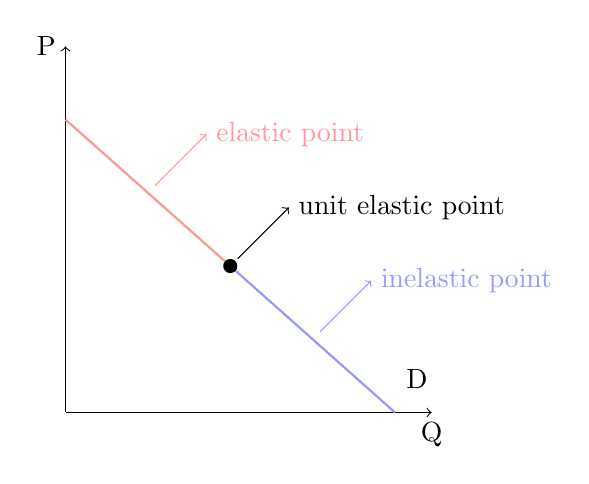
\begin{tikzpicture}[scale=0.93]
    \draw [->] (0,0)--(0,5);
    \draw (0,5)--(0,5) node[left]{P};
    \draw [->] (0,0)--(5,0);
    \draw (5,0)--(5,0) node[below]{Q};
    \draw (0,4)--(4.5,0);
    \draw (4.8,0.2)--(4.8,0.2) node[above]{D};
    \draw [red!40!white,thick] (0,4)--(2.25,2);
    \draw [blue!40!white,thick] (2.25,2)--(4.5,0);
    \node[circle,fill=black,inner sep = 1.8pt] (A1) at (2.25,2) {};
    \draw[->] (2.35,2.1)--(3.05,2.8) node[right]{unit elastic point};
    \draw[->,red!40!white] (1.225,3.1)--(1.925,3.8) node[right]{elastic point};
    \draw[->,blue!40!white] (3.475,1.1)--(4.175,1.8) node[right]{inelastic point};
    
\end{tikzpicture}
\end{figure}

\newpage
\textbf{price elasticity of supply (PES):}
\begin{equation}
    \text{price elasticity of supply (PES)} = {{\%\Delta \text{Q}_S}\over \%\Delta \text{P}}
    \nonumber
\end{equation}

PES is positive because of the law of supply.

\textbf{* if PES<1 }$\Longrightarrow$ price inelastic supply ( $\because$ \%$\Delta$Q$_S$<\%$\Delta$P) 

\textbf{* if PES>1 }$\Longrightarrow$ price elastic supply ( $\because$ \%$\Delta$Q$_S$>\%$\Delta$P)


\textbf{* if PES=0 }$\Longrightarrow$ perfectly price inelastic supply $\Longrightarrow$ $\Delta$P will not affect Q$_S$ ( $\because$ no substitute)

\textbf{* if PES=$+\infty$ }$\Longrightarrow$ perfectly price elastic supply $\Longrightarrow$ $\Delta$P $\rightarrow$ Q$_S$=0 ( $\because$ many substitutes)

\textbf{* if PES=1 }$\Longrightarrow$ unitary price elasticity $\Longrightarrow$ \%$\Delta$Q$_S$ is proportional to \%$\Delta$P

If there's tax on market, the tax burden on producer and consumer depends on the relative price elasticity of demand and supply. The more inelastic side will bear more tax burden.

two examples (tax burden):

\begin{figure}[!h]
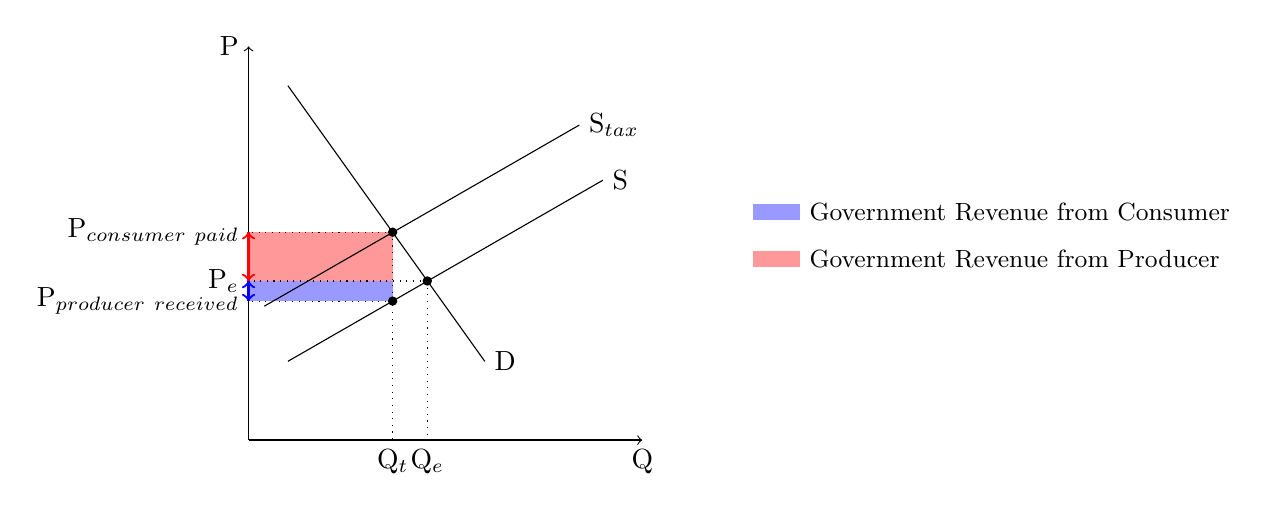
\begin{tikzpicture}
    \fill [red!40!white] (0,2.02)--(0,2.64)--(1.83,2.64)--(1.83,2.02);
    \fill [blue!40!white] (0,1.765)--(0,2.02)--(1.83,2.02)--(1.83,1.765);
    \draw [->] (0,0)--(0,5);
    \draw (0,5)--(0,5) node[left]{P};
    \draw [->] (0,0)--(5,0);
    \draw (5,0)--(5,0) node[below]{Q};
    \draw (0.5,1)--(4.5,3.3) node[right]{S};
    \draw (0.5,4.5)--(3,1) node[right]{D};
    \draw (0.2,1.7)--(4.2,4) node[right]{S$_{tax}$};
    \node[circle,fill=black,inner sep = 1.2pt] (A1) at (2.27,2.02) {};
    \node[circle,fill=black,inner sep = 1.2pt] (A2) at (1.83,2.64) {};
    \node[circle,fill=black,inner sep = 1.2pt] (A3) at (1.83,1.765) {};
    \draw[dotted] (2.27,2.02)--(0,2.02) node[left]{P$_e$};
    \draw[dotted] (1.83,2.64)--(0,2.64) node[left]{P$_{consumer\ paid}$};
    \draw[dotted] (1.83,1.765)--(0,1.765) node[left]{P$_{producer\ received}$};
    \draw[dotted] (2.27,2.02)--(2.27,0) node[below]{Q$_e$};
    \draw[dotted] (1.83,2.64)--(1.83,0) node[below]{Q$_{t}$};
    \fill[blue!40!white] (6.4,3)--(7,3)--(7,2.8)--(6.4,2.8);
    \fill[red!40!white](6.4,2.4)--(7,2.4)--(7,2.2)--(6.4,2.2);
    \draw (7,2.9)--(7,2.9) node[right]{\small Government Revenue from Consumer};
    \draw (7,2.3)--(7,2.3) node[right]{\small Government Revenue from Producer};
    \draw[->,red,thick] (0,2.02)--(0,2.64);
    \draw[->,red,thick] (0,2.64)--(0,2.02);
    \draw[->,blue,thick] (0,1.765)--(0,2.02);
    \draw[->,blue,thick] (0,2.02)--(0,1.765);
\end{tikzpicture}
\caption{PED is more inelastic $\Longrightarrow$ consumer will burden more of tax}
\end{figure}

\begin{figure}[!h]
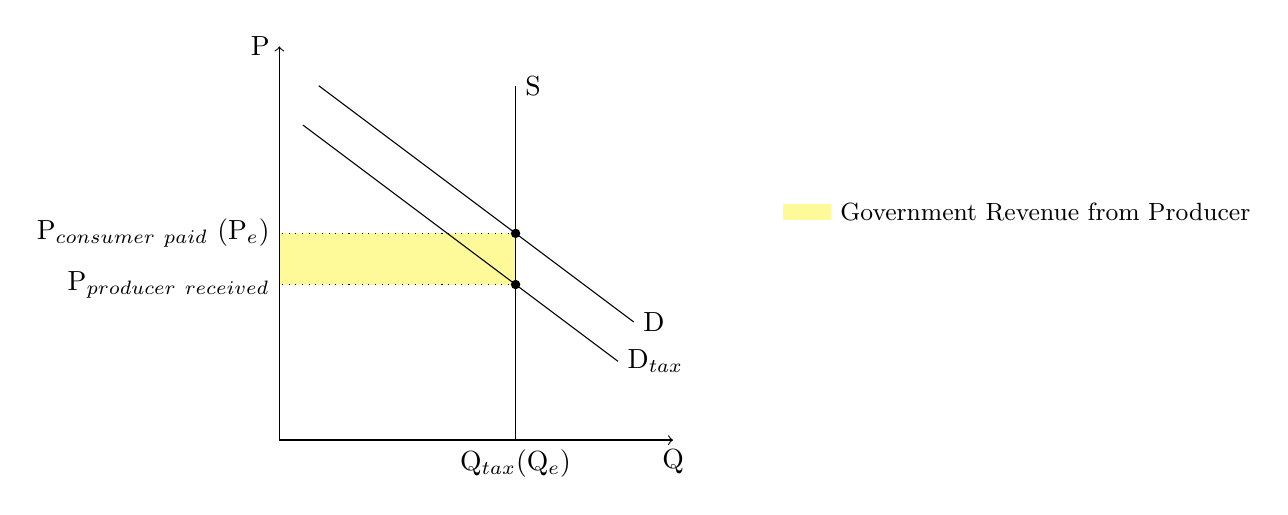
\begin{tikzpicture}
    \fill [yellow!40!white] (0,1.975)--(0,2.625)--(3,2.625)--(3,1.975);
    \draw [->] (0,0)--(0,5);
    \draw (0,5)--(0,5) node[left]{P};
    \draw [->] (0,0)--(5,0);
    \draw (5,0)--(5,0) node[below]{Q};
    \draw (3,0)--(3,4.5) node[right]{S};
    \draw (0.5,4.5)--(4.5,1.5) node[right]{D};
    \draw (0.3,4)--(4.3,1) node[right]{D$_{tax}$};
    \node[circle,fill=black,inner sep = 1.2pt] (A1) at (3,2.625) {};
    \node[circle,fill=black,inner sep = 1.2pt] (A2) at (3,1.975) {};
    \draw[dotted] (3,2.625)--(0,2.625) node[left]{P$_{consumer\ paid}$ (P$_e$)};
    \draw[dotted] (3,1.975)--(0,1.975) node[left]{P$_{producer\ received}$};
    \draw[dotted] (3,2.625)--(3,0) node[below]{Q$_{tax}$(Q$_e$)};
    \fill[yellow!40!white] (6.4,3)--(7,3)--(7,2.8)--(6.4,2.8);
    \draw (7,2.9)--(7,2.9) node[right]{\small Government Revenue from Producer};


\end{tikzpicture}
\caption{PES is perfectly inelastic $\Longrightarrow$ producer will burden all of tax}
\end{figure}

\newpage
\noindent

\begin{lemma}
    The DWL of elastic market is greater than the DWL of inelastic market.
\end{lemma}

%\begin{proof}
 %   Since the $\text{DWL} = {\displaystyle{1\over2}}\times \text{per unit tax}\times \Delta \text{Q}$
%\end{proof}

\begin{proof}
We start from the calculation of DWL:
\[
\text{DWL} = {\displaystyle{1\over2}}\times \text{per unit tax}\times \Delta \text{Q} = {\displaystyle{1\over2}}\times \text{per unit tax} \times (Q_e-Q_{tax})
\]

Next, we know that the elasticity will affect the change in quantity $\Delta$Q, and the more elastic the market is, the greater the change in quantity will be.:
\[
\text{DWL}_{more\ elastic}>\text{DWL}_{less\ elastic}
\]

Thus, the result follows.
\end{proof}


\textbf{Cross-price elasticity of demand (XED):}
\begin{equation}
    \text{cross-price elasticity of demand (XED)} = {{\%\Delta \text{Q}_D\ \text{of good A}}\over \%\Delta \text{P}\ \text{of good B}}
    \nonumber
\end{equation}

* if XED > 0 $\Longrightarrow$ good A and good B are substitutes ( $\because$ price of B $\uparrow$ $\longrightarrow$ demand for A $\uparrow$)    

* if XED < 0 $\Longrightarrow$ good A and good B are complements ( $\because$ price of B $\uparrow$ $\longrightarrow$ demand for A $\downarrow$)

\textbf{Income elasticity of demand (YED):}
\begin{equation}
    \text{income elasticity of demand (YED)} = {{\%\Delta \text{Q}_D}\over \%\Delta \text{income}}
    \nonumber
\end{equation}

* if YED < 0 $\Longrightarrow$ inferior good ( $\because$ income $\uparrow$ $\longrightarrow$ demand $\downarrow$)

* if 0 <YED < 1 $\Longrightarrow$ necessity (normal good) ( $\because$ income $\uparrow$ $\longrightarrow$ demand $\uparrow$)

* if YED > 1 $\Longrightarrow$ luxury (normal good) ( $\because$ income $\uparrow$ $\longrightarrow$ demand $\uparrow$)

\newpage
\section{Trade Barriers}

Government may intervene in the market to protect domestic producers from foreign competition by imposing trade barriers, such as tariffs and quotas. \textbf{(Trade Protectionism)}

\textbf{World Price (WP)}: the price trade in the international market (assume the country is a price taker in the world market $\Longrightarrow$ horizontal).

\begin{figure}[!h]
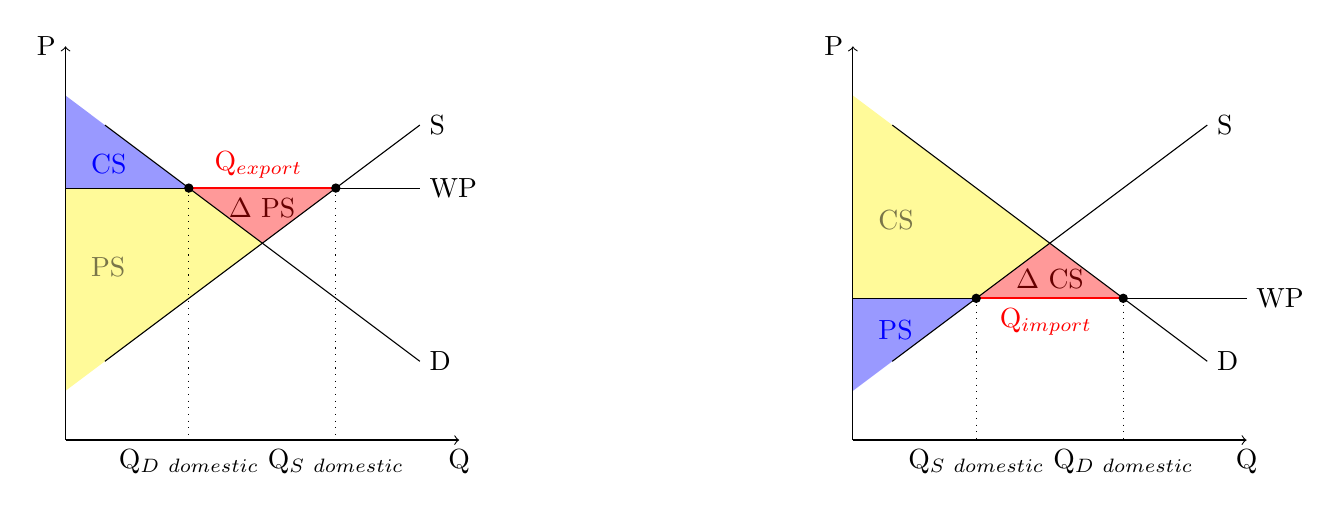
\begin{tikzpicture}
    \fill [blue!40!white] (0,3.2)--(1.566,3.2)--(0,4.375);
    \fill [yellow!40!white] (3.433,3.2)--(0,0.625)--(0,3.2);
    \fill [red!40!white] (3.433,3.2)--(1.566,3.2)--(2.5,2.5);
    \draw [->] (0,0)--(0,5);
    \draw (0,5)--(0,5) node[left]{P};
    \draw [->] (0,0)--(5,0);
    \draw (5,0)--(5,0) node[below]{Q};
    \draw (0.5,1)--(4.5,4) node[right]{S};
    \draw (0.5,4)--(4.5,1) node[right]{D};
    \draw (0,3.2)--(4.5,3.2) node[right]{WP};
    \draw[red,thick](3.433,3.2)--(1.566,3.2);
    \draw [red](2.45,3.2)--(2.45,3.2) node[above]{Q$_{export}$};
    \node[circle,fill=black,inner sep = 1.2pt] (A1) at (3.433,3.2) {};
    \node[circle,fill=black,inner sep = 1.2pt] (A2) at (1.566,3.2) {};
    \draw[dotted] (3.433,3.2)--(3.433,0) node[below]{Q$_{S\ domestic}$};
    \draw[dotted] (1.566,3.2)--(1.566,0) node[below]{Q$_{D\ domestic}$};
    \draw (0.2,3.5)--(0.2,3.5) node[right,blue]{CS};
    \draw (0.2,2.2)--(0.2,2.2) node[right,yellow!40!black]{PS};
    \draw (1.95,2.95)--(1.95,2.95) node[right,red!40!black]{$\Delta$ PS};


    \fill [blue!40!white] (10,0.625)--(11.566,1.8)--(10,1.8);
    \fill [yellow!40!white] (10,4.375)--(13.433,1.8)--(10,1.8);
    \fill [red!40!white] (13.433,1.8)--(11.566,1.8)--(12.5,2.5);
    \draw [->] (10,0)--(10,5);
    \draw (10,5)--(10,5) node[left]{P};
    \draw [->] (10,0)--(15,0);
    \draw (15,0)--(15,0) node[below]{Q};
    \draw (10.5,1)--(14.5,4) node[right]{S};
    \draw (10.5,4)--(14.5,1) node[right]{D};
    \draw (10,1.8)--(15,1.8) node[right]{WP};
    \draw[red,thick](13.433,1.8)--(11.566,1.8);
    \draw [red](12.45,1.8)--(12.45,1.8) node[below]{Q$_{import}$};
    \node[circle,fill=black,inner sep = 1.2pt] (A1) at (13.433,1.8) {};
    \node[circle,fill=black,inner sep = 1.2pt] (A2) at (11.566,1.8) {};
    \draw[dotted] (13.433,1.8)--(13.433,0) node[below]{Q$_{D\ domestic}$};
    \draw[dotted] (11.566,1.8)--(11.566,0) node[below]{Q$_{S\ domestic}$};
    \draw (10.2,2.8)--(10.2,2.8) node[right,yellow!40!black]{CS};
    \draw (10.2,1.4)--(10.2,1.4) node[right,blue]{PS};
    \draw (11.95,2.05)--(11.95,2.05) node[right,red!40!black]{$\Delta$ CS};


    

\end{tikzpicture}
\end{figure}
\subsection{Tariff}

\textbf{Tariff} is a tax on imported goods, which increases the price of imported goods and reduces the quantity of imports.

\begin{figure}[!h]
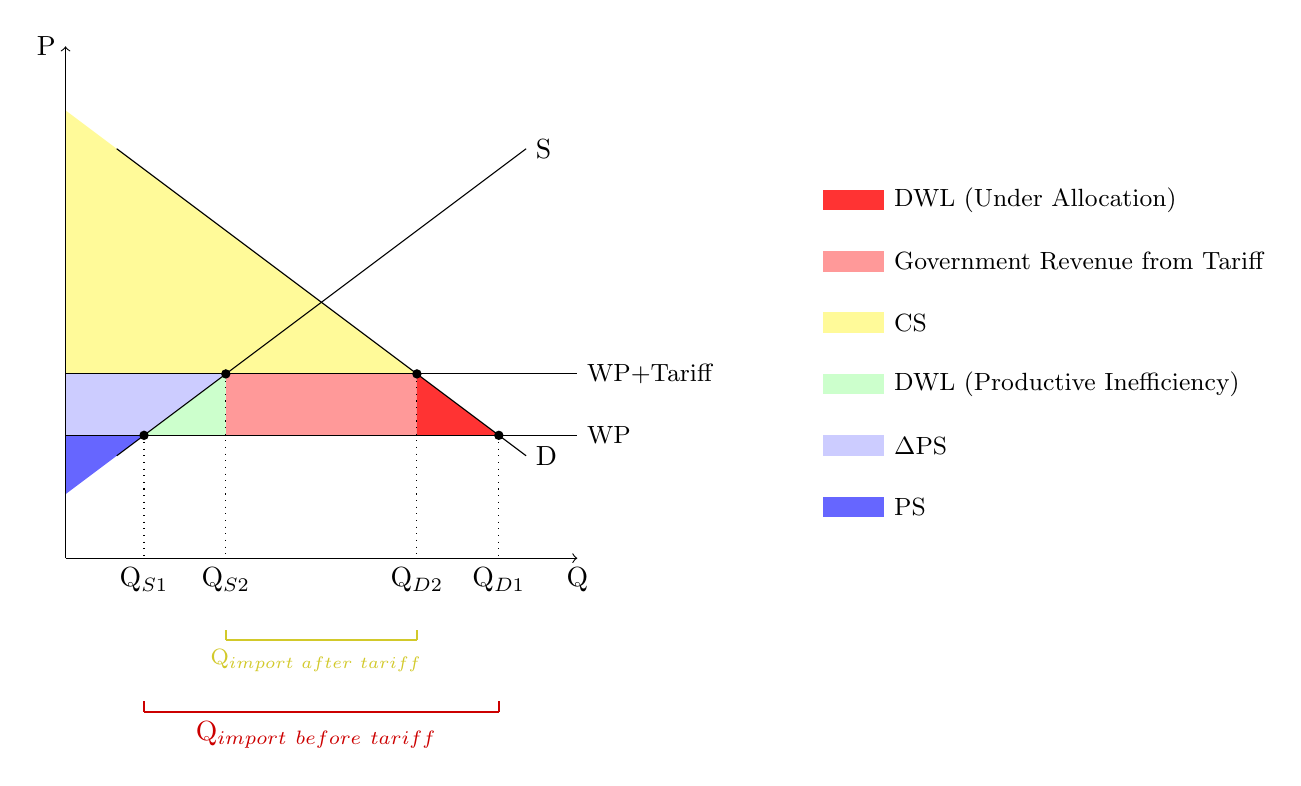
\begin{tikzpicture}[scale=1.3]
    \fill [blue!60!white] (0,1.2)--(0.767,1.2)--(0,0.625);
    \fill [blue!20!white] (0,1.2)--(0.767,1.2)--(1.566,1.8)--(0,1.8);
    \fill [yellow!40!white] (0,1.8)--(3.433,1.8)--(0,4.375);
    \fill [red!40!white] (1.566,1.2)--(1.566,1.8)--(3.433,1.8)--(3.433,1.2);
    \fill [green!20!white] (1.566,1.2)--(1.566,1.8)--(0.767,1.2);
    \fill [red!80!white] (3.433,1.2)--(3.433,1.8)--(4.233,1.2);
    \draw [->] (0,0)--(0,5);
    \draw (0,5)--(0,5) node[left]{P};
    \draw [->] (0,0)--(5,0);
    \draw (5,0)--(5,0) node[below]{Q};
    \draw (0.5,1)--(4.5,4) node[right]{S};
    \draw (0.5,4)--(4.5,1) node[right]{D};
    \draw (0,1.2)--(5,1.2) node[right]{\small WP};
    \draw[red!80!black,thick](0.767,-1.5)--(4.233,-1.5);
    \draw[red!80!black,thick](0.767,-1.5)--(0.767,-1.4);
    \draw[red!80!black,thick](4.233,-1.5)--(4.233,-1.4);
    \draw [red!80!black](2.45,-1.5)--(2.45,-1.5) node[below]{Q$_{import\ before\ tariff}$};
    \node[circle,fill=black,inner sep = 1.2pt] (A1) at (0.767,1.2) {};
    \node[circle,fill=black,inner sep = 1.2pt] (A2) at (4.233,1.2) {};
    \draw[dotted] (4.233,1.2)--(4.233,0) node[below]{Q$_{D1}$};
    \draw[dotted] (0.767,1.2)--(0.767,0) node[below]{Q$_{S1}$};
    \draw (0,1.8)--(5,1.8) node[right]{\small WP+Tariff};
    \node[circle,fill=black,inner sep = 1.2pt] (A1) at (3.433,1.8) {};
    \node[circle,fill=black,inner sep = 1.2pt] (A2) at (1.566,1.8) {};
    \draw[dotted] (3.433,1.8)--(3.433,0) node[below]{Q$_{D2}$};
    \draw[dotted] (1.566,1.8)--(1.566,0) node[below]{Q$_{S2}$};
    \draw[yellow!80!black,thick](1.566,-0.8)--(3.433,-0.8);
    \draw[yellow!80!black,thick](1.566,-0.8)--(1.566,-0.7);
    \draw[yellow!80!black,thick](3.433,-0.8)--(3.433,-0.7);
    \draw [yellow!80!black](2.45,-0.8)--(2.45,-0.8) node[below]{\footnotesize Q$_{import\ after\ tariff}$};
    \fill[red!80!white](7.4,3.6)--(8,3.6)--(8,3.4)--(7.4,3.4);
    \fill[red!40!white] (7.4,3)--(8,3)--(8,2.8)--(7.4,2.8);
    \fill[yellow!40!white](7.4,2.4)--(8,2.4)--(8,2.2)--(7.4,2.2);
    \fill[green!20!white](7.4,1.8)--(8,1.8)--(8,1.6)--(7.4,1.6);
    \fill[blue!20!white] (7.4,1.2)--(8,1.2)--(8,1)--(7.4,1);
    \fill[blue!60!white](7.4,0.6)--(8,0.6)--(8,0.4)--(7.4,0.4);
    
    \draw (8,3.5)--(8,3.5) node[right]{\small DWL (Under Allocation)};
    \draw (8,2.9)--(8,2.9) node[right]{\small Government Revenue from Tariff};
    \draw (8,2.3)--(8,2.3) node[right]{\small CS};
    \draw (8,1.7)--(8,1.7) node[right]{\small DWL (Productive Inefficiency)};
    \draw (8,1.1)--(8,1.1) node[right]{\small $\Delta$PS};
    \draw (8,0.5)--(8,0.5) node[right]{\small PS};

    
\end{tikzpicture}
\caption{Domestic market after tariff}
\end{figure}

\subsection{Quota}

\textbf{Quota} is a limit on the quantity of imported goods, which reduces the quantity of imports and increases the price of imported goods.

\begin{figure}[!h]
    \centering
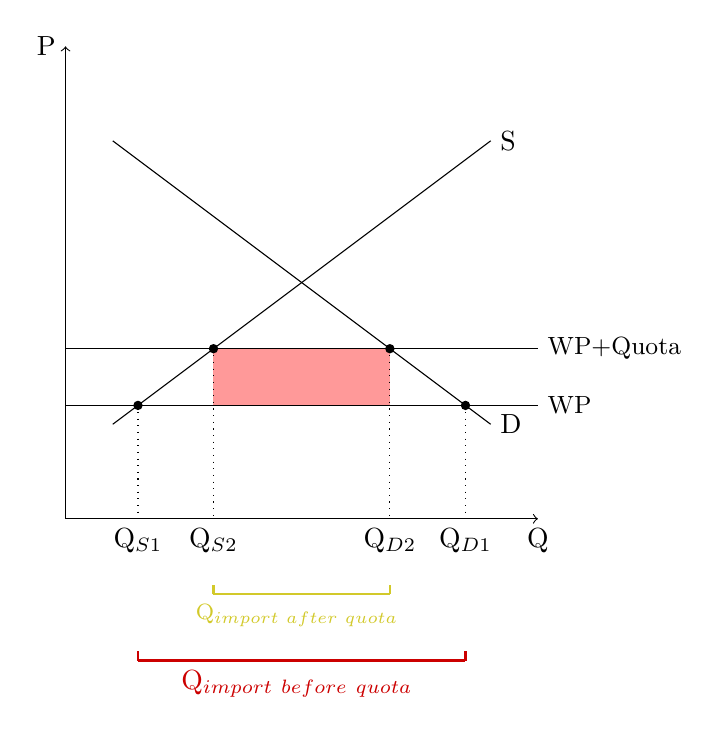
\begin{tikzpicture}[scale=1.2]
    \fill [red!40!white] (1.566,1.2)--(1.566,1.8)--(3.433,1.8)--(3.433,1.2);
    \draw [->] (0,0)--(0,5);
    \draw (0,5)--(0,5) node[left]{P};
    \draw [->] (0,0)--(5,0);
    \draw (5,0)--(5,0) node[below]{Q};
    \draw (0.5,1)--(4.5,4) node[right]{S};
    \draw (0.5,4)--(4.5,1) node[right]{D};
    \draw (0,1.2)--(5,1.2) node[right]{\small WP};
    \draw[red!80!black,thick](0.767,-1.5)--(4.233,-1.5);
    \draw[red!80!black,thick](0.767,-1.5)--(0.767,-1.4);
    \draw[red!80!black,thick](4.233,-1.5)--(4.233,-1.4);
    \draw [red!80!black](2.45,-1.5)--(2.45,-1.5) node[below]{Q$_{import\ before\ quota}$};
    \node[circle,fill=black,inner sep = 1.2pt] (A1) at (0.767,1.2) {};
    \node[circle,fill=black,inner sep = 1.2pt] (A2) at (4.233,1.2) {};
    \draw[dotted] (4.233,1.2)--(4.233,0) node[below]{Q$_{D1}$};
    \draw[dotted] (0.767,1.2)--(0.767,0) node[below]{Q$_{S1}$};
    \draw (0,1.8)--(5,1.8) node[right]{\small WP+Quota};
    \node[circle,fill=black,inner sep = 1.2pt] (A1) at (3.433,1.8) {};
    \node[circle,fill=black,inner sep = 1.2pt] (A2) at (1.566,1.8) {};
    \draw[dotted] (3.433,1.8)--(3.433,0) node[below]{Q$_{D2}$};
    \draw[dotted] (1.566,1.8)--(1.566,0) node[below]{Q$_{S2}$};
    \draw[yellow!80!black,thick](1.566,-0.8)--(3.433,-0.8);
    \draw[yellow!80!black,thick](1.566,-0.8)--(1.566,-0.7);
    \draw[yellow!80!black,thick](3.433,-0.8)--(3.433,-0.7);
    \draw [yellow!80!black](2.45,-0.8)--(2.45,-0.8) node[below]{\footnotesize Q$_{import\ after\ quota}$};
\end{tikzpicture}
\end{figure}

\newpage
\section{Costs of Production}
\noindent

\textbf{explicit cost} (EC) $\longrightarrow$ (accounting cost): how much money you spent

\textbf{implicit cost} (IC) $\longrightarrow$ (opportunity cost, hidden cost): how much you give up

calculation of profit:
\begin{equation}
\text{Profit} = \text{total revenue} - \text{total cost} = \text{TR} - \text{TC}
\nonumber
\end{equation}

economic profit (EP) $\longrightarrow$ TR $-$ (EC $+$ IC)

accounting profit (AP) $\longrightarrow$ TR $-$ EC

normal profit $\longrightarrow$ EP = 0. If a firm is profitable $\Longrightarrow$ TR > EC + IC (EP > 0).

\textbf{* Marginal Analysis} profit maximization occurs:

\begin{equation}
    (\text{TR}-\text{TC})' = 0 \Longrightarrow \text{TR}' = \text{TC}' \Longrightarrow \text{MR} = \text{MC}
    \nonumber
\end{equation}

\subsection{Firm's Production}
\noindent

\textbf{production function}: the relationship between quantity of inputs and quantity of output.

\textbf{total product} (TP): the total quantity of output produced by a given quantity of input.

\textbf{marginal product} (MP): the additional quantity of output produced by using one more unit of input.

\textcolor{blue}{Diminishing marginal product:} the marginal product of an input decreases as the quantity of the input increases.

\begin{figure}[!h]
    \centering
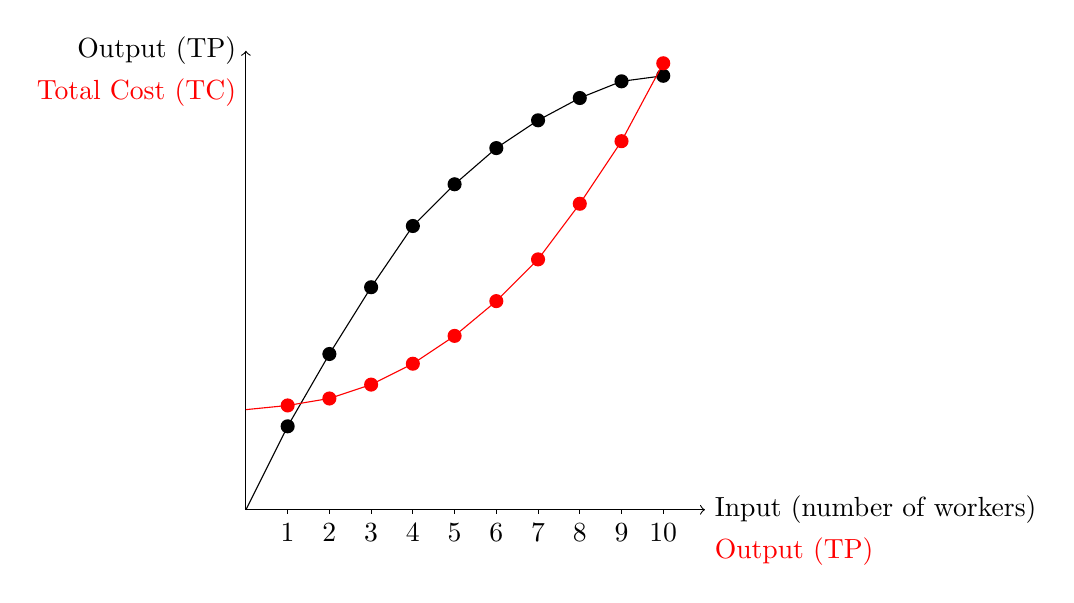
\begin{tikzpicture}[scale=0.53]
    \draw [->] (0,0)--(0,11);
    \draw (0,11)--(0,11) node[left]{Output (TP)};
    \draw[red] (0,10)--(0,10) node[left]{Total Cost (TC)};
    \draw [->] (0,0)--(11,0);
    \draw (11,0)--(11,0) node[right]{Input (number of workers)};
    \draw[red] (11,-1)--(11,-1) node[right]{Output (TP)};
    \foreach \x in {1,2,3,4,5,6,7,8,9,10}
{
    \draw (\x,0)--(\x,-0.1) node[below]{\x};
}
    \node[circle,fill=black,inner sep = 1.8pt] (A1) at (1,2) {};
    \node[circle,fill=black,inner sep = 1.8pt] (A2) at (2,3.733) {};
    \node[circle,fill=black,inner sep = 1.8pt] (A3) at (3,5.333) {};
    \node[circle,fill=black,inner sep = 1.8pt] (A4) at (4,6.8) {};
    \node[circle,fill=black,inner sep = 1.8pt] (A5) at (5,7.8) {};
    \node[circle,fill=black,inner sep = 1.8pt] (A6) at (6,8.667) {};
    \node[circle,fill=black,inner sep = 1.8pt] (A7) at (7,9.333) {};
    \node[circle,fill=black,inner sep = 1.8pt] (A8) at (8,9.867) {};
    \node[circle,fill=black,inner sep = 1.8pt] (A9) at (9,10.267) {};
    \node[circle,fill=black,inner sep = 1.8pt] (A10) at (10,10.4) {};
    \draw (0,0)--(1,2)--(2,3.733)--(3,5.333)--(4,6.8)--(5,7.8)--(6,8.667)--(7,9.333)--(8,9.867)--(9,10.267)--(10,10.4);




    \node[circle,fill=red,inner sep = 1.8pt] (B1) at (1,2.5) {};
    \node[circle,fill=red,inner sep = 1.8pt] (B2) at (2,2.667) {};
    \node[circle,fill=red,inner sep = 1.8pt] (B3) at (3,3) {};
    \node[circle,fill=red,inner sep = 1.8pt] (B4) at (4,3.5) {};
    \node[circle,fill=red,inner sep = 1.8pt] (B5) at (5,4.167) {};
    \node[circle,fill=red,inner sep = 1.8pt] (B6) at (6,5) {};
    \node[circle,fill=red,inner sep = 1.8pt] (B7) at (7,6) {};
    \node[circle,fill=red,inner sep = 1.8pt] (B8) at (8,7.333) {};
    \node[circle,fill=red,inner sep = 1.8pt] (B9) at (9,8.833) {};
    \node[circle,fill=red,inner sep = 1.8pt] (B10) at (10,10.7) {};
    \draw[red] (0,2.4)--(1,2.5)--(2,2.667)--(3,3)--(4,3.5)--(5,4.167)--(6,5)--(7,6)--(8,7.333)--(9,8.833)--(10,10.7);
\end{tikzpicture}
\end{figure}

From the graph, we can see that the total product (TP) increases at a decreasing rate as the input increases, which illustrates the law of diminishing marginal product. 

$\Longrightarrow$ The shape of marginal product will determine the marginal cost curve.

\subsection{Cost Curve}

Relationship between total cost (TC), fixed cost (FC), variable cost (VC): \textbf{TC = FC + VC}

\begin{figure}[!h]
    \centering
\begin{tikzpicture}[scale=0.7]
    \draw [->] (0,0)--(0,7);
    \draw (0,7)--(0,7) node[left]{Cost};
    \draw [->] (0,0)--(11,0);
    \draw (11,0)--(11,0) node[right]{Output};
    \draw[red] (0,2)--(10,5.5) node[right]{TC};
    \draw[blue] (0,2)--(10,2) node[right]{FC};
    \draw[green] (0,0)--(10,3.5) node[right]{VC};
    
\end{tikzpicture}    
\end{figure}

\textbf{Average:}
\begin{equation}
\begin{aligned}
    \text{average fixed cost (AFC)} &= {\text{FC}\over \text{Q}} \Longrightarrow \text{always decreasing}\\
    \text{average variable cost (AVC)} &= {\text{VC}\over \text{Q}} \Longrightarrow \text{U-shaped}\\
    \text{average total cost (ATC)} &= {\text{TC}\over \text{Q}} = {\text{FC}+\text{VC}\over \text{Q}} = \text{AFC} + \text{AVC} \Longrightarrow \text{U-shaped}
    \nonumber
\end{aligned}
\end{equation}

\textbf{Marginal:}
\begin{equation}
\begin{aligned}
    \text{marginal cost (MC)} &= {\Delta \text{TC} \over \Delta \text{Q}} = {\Delta \text{VC} \over \Delta \text{Q}} \Longrightarrow \text{U-shaped}\\
    \nonumber
\end{aligned}
\end{equation}

Relationship between \textbf{Average} and \textbf{Marginal:} 

1. When MC < ATC (or AVC) $\Longrightarrow$ ATC (or AVC) $\downarrow$

2. When MC > ATC (or AVC) $\Longrightarrow$ ATC (or AVC) $\uparrow$

3. When MC = ATC (or AVC) $\Longrightarrow$ ATC (or AVC) is at its minimum point

\begin{figure}
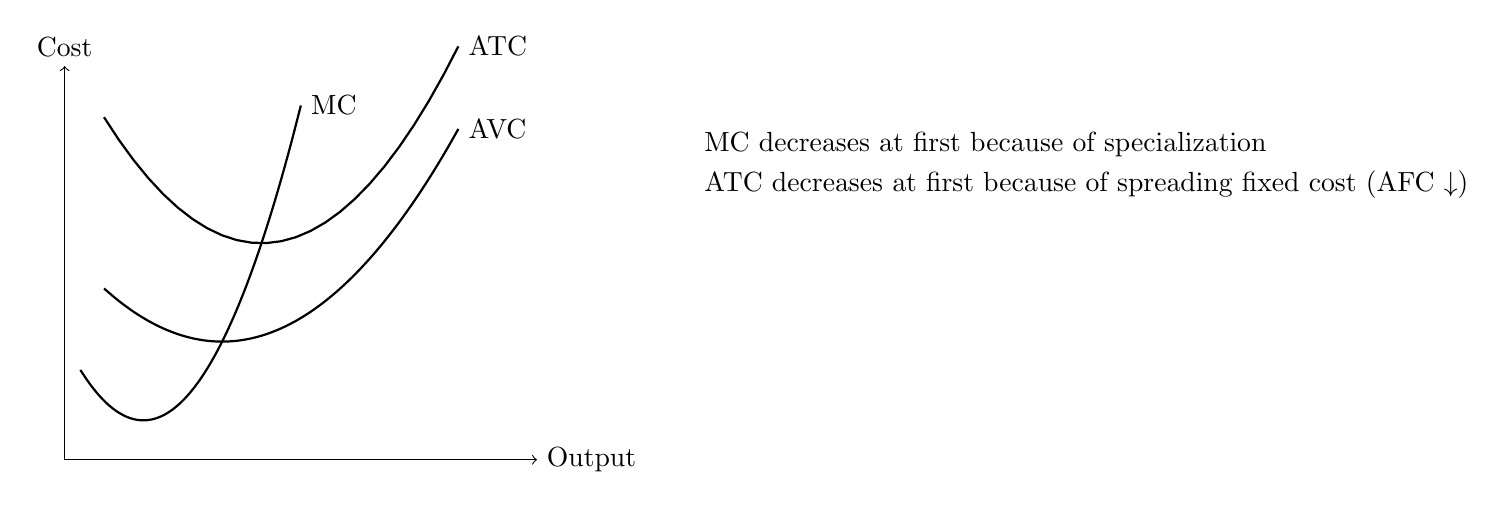
\begin{tikzpicture}

\draw[->] (0,0)--(6,0) node[right]{Output};
\draw[->] (0,0)--(0,5) node[above]{Cost};

\draw[thick, domain=0.2:3, smooth]
    plot (\x, {(\x-1)^2 + 0.5}) node[right]{MC};

\draw[thick, domain=0.5:5, smooth]
    plot (\x, {0.3*(\x-2)^2 + 1.5}) node[right]{AVC};
\draw[thick, domain=0.5:5]
    plot (\x, {0.4*(\x-2.5)^2 + 2.75}) node[right]{ATC}; 

    \draw (8,4)--(8,4) node[right]{MC decreases at first because of specialization};
    \draw (8,3.5)--(8,3.5) node[right]{ATC decreases at first because of spreading fixed cost (AFC $\downarrow$)};

\end{tikzpicture}
\end{figure}

\newpage 

$\because$ \textbf{Profit} = TR $-$ TC = (P $-$ ATC) $\times$ Q 

$\therefore$ if P > ATC $\Longrightarrow$ economic profit > 0 

$\therefore$ if P = ATC $\Longrightarrow$ economic profit = 0 (normal profit)

$\therefore$ if P < ATC $\Longrightarrow$ economic profit < 0\\

In the short run: ATC does not make a lot sense because FC is sunk cost in the short run. $\longrightarrow$ the decision to shut down or not should be based on AVC, not ATC (P = AVC is the breakdown point in the short run).\\

\begin{tabular}{|c|c|}
\hline
\textbf{Short Run} & \textbf{Long Run} \\
\hline
at least one fixed input (land, building, equipment, capital) & all inputs are variable \\
\hline
\end{tabular}\\

In the long run: 

\begin{figure}[!h]
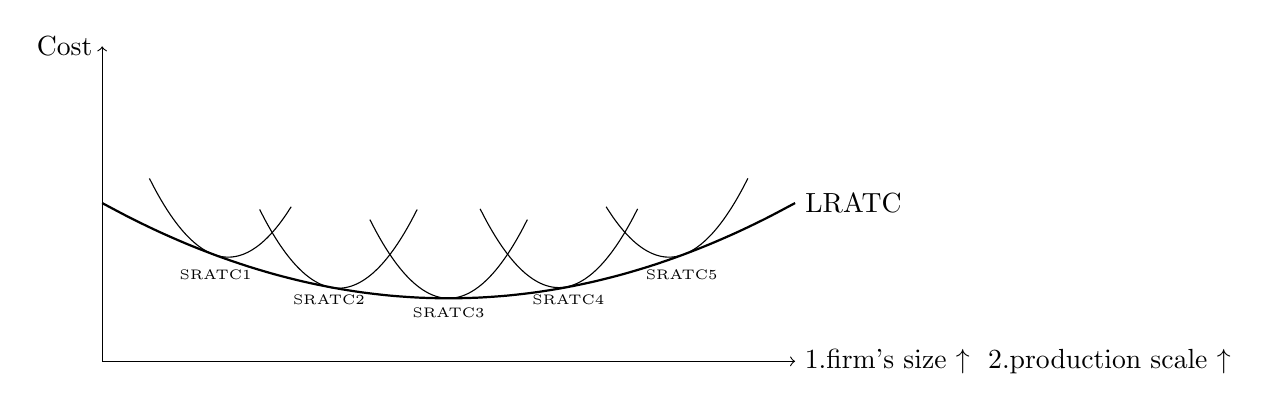
\begin{tikzpicture}[scale=0.8]
    \draw [->] (0,0)--(0,5);
    \draw (0,5)--(0,5) node[left]{Cost};
    \draw [->] (0,0)--(11,0);
    \draw (11,0)--(11,0) node[right]{1.firm's size $\uparrow$\ \ 2.production scale $\uparrow$};
\draw[thick, domain=0:11, smooth]
    plot (\x, {0.05*(\x-5.5)^2 + 1}) node[right]{LRATC};
\draw[domain=4.25:6.75, smooth]
    plot (\x, {0.8*(\x-5.5)^2 + 1});
\draw[domain=0.75:3, smooth]
    plot (\x, {0.8*(\x-2)^2 + 1.6533});
\draw[domain=2.5:5, smooth]
    plot (\x, {0.8*(\x-3.75)^2 + 1.16});
\draw[domain=6:8.5, smooth]
    plot (\x, {0.8*(\x-7.25)^2 + 1.17});
\draw[domain=8:10.25, smooth]
    plot (\x, {0.8*(\x-9)^2 + 1.6533});
    \draw (1.8,1.6)--(1.8,1.6) node[below]{\tiny SRATC1};
    \draw (3.6,1.2)--(3.6,1.2) node[below]{\tiny SRATC2};
    \draw (5.5,1)--(5.5,1) node[below]{\tiny SRATC3};
    \draw (7.4,1.2)--(7.4,1.2) node[below]{\tiny SRATC4};
    \draw (9.2,1.6)--(9.2,1.6) node[below]{\tiny SRATC5};
\end{tikzpicture}    
\end{figure}

\begin{figure}[!h]
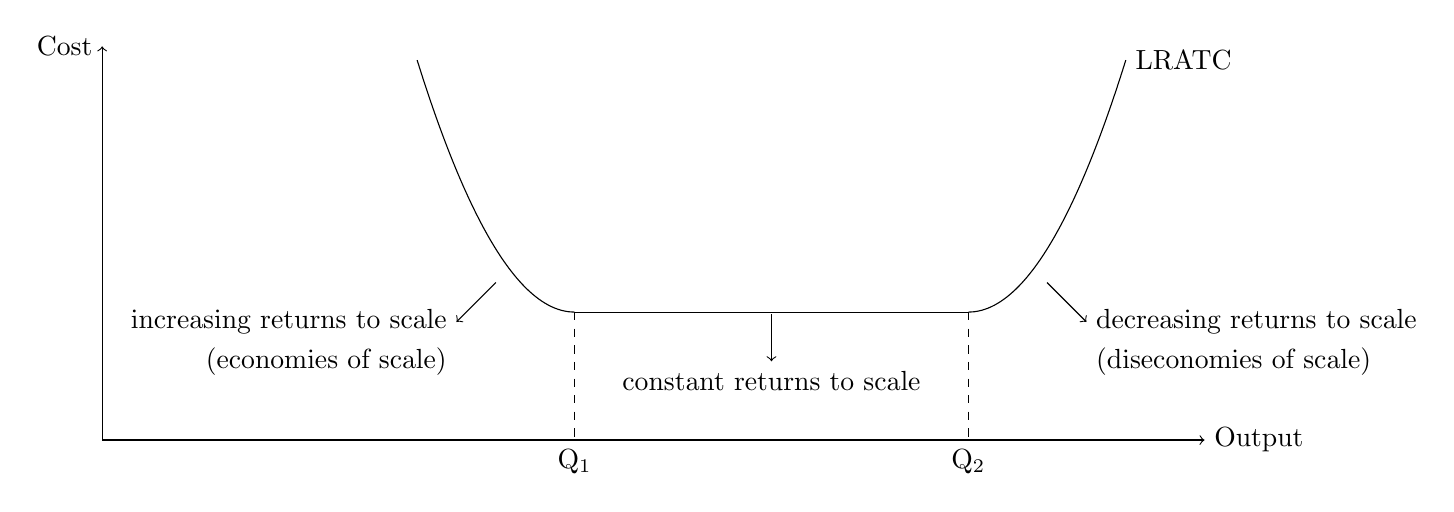
\begin{tikzpicture}
    \draw [->] (-3,0)--(-3,5);
    \draw (-3,5)--(-3,5) node[left]{Cost};
    \draw [->] (-3,0)--(11,0);
    \draw (11,0)--(11,0) node[right]{Output};
\draw[domain=1:3, smooth]
    plot (\x, {0.8*(\x-3)^2 + 1.625});
\draw[domain=8:10, smooth]
    plot (\x, {0.8*(\x-8)^2 + 1.625}) node[right]{LRATC};
    \draw (3,1.625)--(8,1.625);
    \draw [dashed](3,1.625)--(3,0) node[below]{Q$_1$};
    \draw [dashed](8,1.625)--(8,0) node[below]{Q$_2$};
    \draw[->] (5.5,1.6)--(5.5,1);
    \draw (5.5,1)--(5.5,1) node[below]{constant returns to scale};
    \draw[->] (2,2)--(1.5,1.5) node[left]{increasing returns to scale};
    \draw (1.5,1)--(1.5,1) node[left]{(economies of scale)};
    \draw[->] (9,2)--(9.5,1.5) node[right]{decreasing returns to scale};
    \draw (9.5,1)--(9.5,1) node[right]{(diseconomies of scale)};
\end{tikzpicture}
\end{figure}

\begin{tabular}{|c|c|}
\hline
\textbf{Increasing Returns to Scale} (Economies of Scale) & \textbf{Decreasing Returns to Scale} (Diseconomies of Scale) \\
\hline
LRATC $\downarrow$ $\Longrightarrow$ Q/plant size $\uparrow$ & LRATC $\uparrow$ $\Longrightarrow$ Q/plant size $\downarrow$ \\
\hline
\textbf{Reason:} specialization of labor, capital & management inefficiency, communication problems \\
\hline
\end{tabular}


\newpage
\section{Perfect \& Imperfect Competition Markets}
Preview (perfect competition, monopoly, monopolistic competition, oligopoly)\\

\begin{figure}[!h]
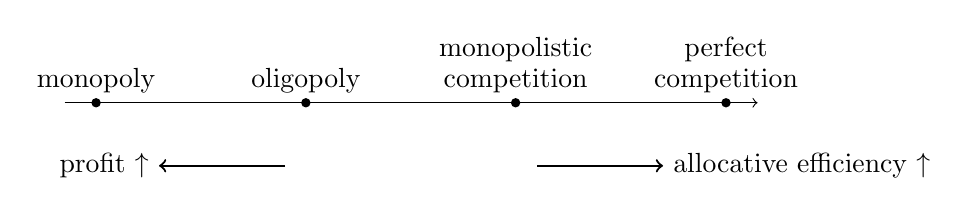
\begin{tikzpicture}[scale=0.8]
    \draw [->](-0.5,0)--(10.5,0);
    \node [circle,fill=black,inner sep = 1.2pt] (A1) at (0,0) {};
    \node [circle,fill=black,inner sep = 1.2pt] (A2) at (3.33,0) {};
    \node [circle,fill=black,inner sep = 1.2pt] (A3) at (6.66,0) {};
    \node [circle,fill=black,inner sep = 1.2pt] (A4) at (10,0) {};
    \draw (0,0)--(0,0) node[above]{monopoly};
    \draw (3.33,0)--(3.33,0) node[above]{oligopoly};
    \draw (6.66,0.5)--(6.66,0.5) node[above]{monopolistic};
    \draw (6.66,0)--(6.66,0) node[above]{competition};
    \draw (10,0.5)--(10,0.5) node[above]{perfect};
    \draw (10,0)--(10,0) node[above]{competition};
    \draw[thick,->] (7,-1)--(9,-1) node[right]{allocative efficiency $\uparrow$};
    \draw[thick,->] (3,-1)--(1,-1) node[left]{profit $\uparrow$};
    
\end{tikzpicture}
\end{figure}

\subsection{Perfect Competition}
\noindent
for any single seller or buyer, they will have no influence on the market price $\Longrightarrow$ (price taker).

\textbf{static assumption: } 1. identical products (perfect substitutes)\ \ \ 2. many firms

\textbf{dynamic assumption: } free entry and exit (long run equilibrium)

\textbf{*(flat demand)} Since the market determines the price, the demand curve for each firm is perfectly elastic (horizontal) at the market price. \textbf{*(MR=P)} Since the price at all units is the same, the marginal revenue (MR) is equal to the price (P) for each unit sold.

\begin{figure}[!h]
    \centering
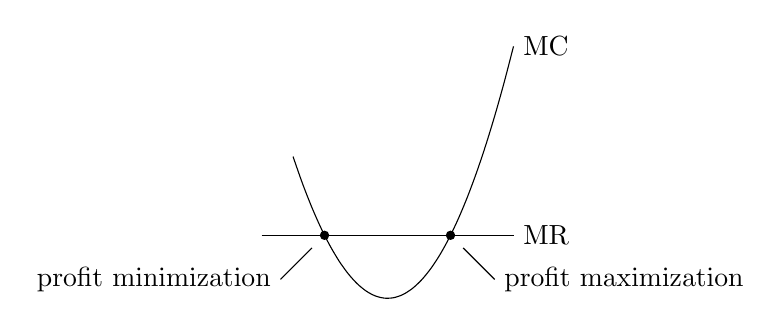
\begin{tikzpicture}[scale=0.8]
\draw[domain=-0.5:3, smooth]
    plot (\x, {(\x-1)^2 + 0.5}) node[right]{MC};
    \draw (-1,1.5)--(3,1.5) node[right]{MR};
    \node [circle,fill=black,inner sep = 1.2pt] (A1) at (0,1.5) {};
    \node [circle,fill=black,inner sep = 1.2pt] (A2) at (2,1.5) {};
    \draw (-0.2,1.3)--(-0.7,0.8) node[left]{profit minimization};
    \draw (2.2,1.3)--(2.7,0.8) node[right]{profit maximization};


\end{tikzpicture}
\end{figure}

\begin{lemma}
    In the short run, since the firms are chasing profit maximization, the equilibrium output is determined by the intersection of MR and MC \textbf{(MR=MC)}.
\end{lemma}

\begin{figure}[!h]
    \centering
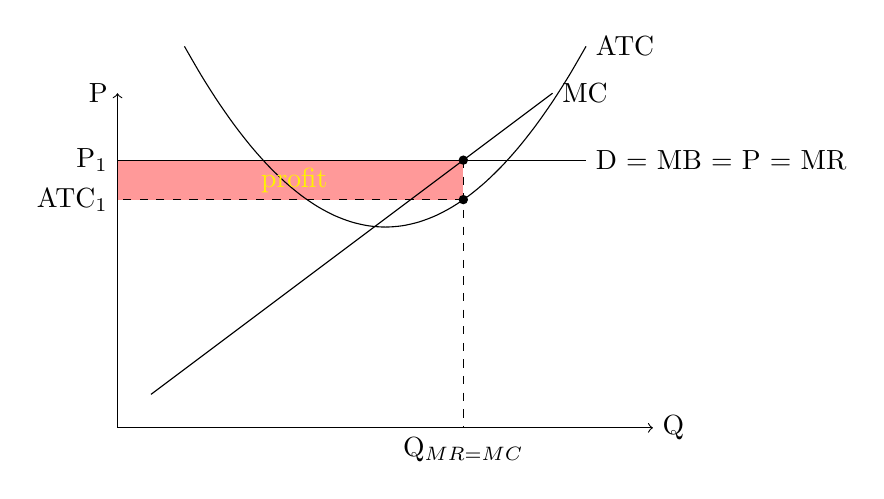
\begin{tikzpicture}[scale=0.85]
    \fill [red!40!white] (0,3.41)--(0,4)--(5.1667,4)--(5.1667,3.41);
    \draw [->] (0,0)--(0,5);
    \draw (0,5)--(0,5) node[left]{P};
    \draw [->] (0,0)--(8,0);
    \draw (8,0)--(8,0) node[right]{Q};
    \draw (0,4)--(7,4) node[right]{D $=$ MB $=$ P $=$ MR};
    \draw (0.5,0.5)--(6.5,5) node[right]{MC};
    \node[circle,fill=black,inner sep = 1.2pt] (A1) at (5.1667,4) {};
\draw[domain=1:7, smooth]
    plot (\x, {0.3*(\x-4)^2 + 3}) node[right]{ATC};
    \draw[dashed] (5.1667,4)--(5.1667,0) node[below]{Q$_{MR=MC}$};
    \node [circle,fill=black,inner sep = 1.2pt] (A2) at (5.1667,3.41) {};
    \draw[dashed] (5.1667,3.41)--(0,3.41) node[left]{ATC$_1$};
    \draw (0,4)--(0,4) node[left]{P$_1$};
    \draw [yellow](2,3.7)--(2,3.7) node[right]{profit};
\end{tikzpicture}
\caption{perfect competition market in short run}
\end{figure}

\textbf{allocative efficiency:} maximized wealth $=$ maximized TS $=$ maximized CS $+$ PS $\Longrightarrow$ \textbf{MB = MC}

\begin{proof}
    the firms chase profit maximization $\Longrightarrow$ MR = MC. Since the demand curve is perfectly elastic, P = MR $\Longrightarrow$ P = MC $\Longrightarrow$ MB = MC $\Longrightarrow$ allocative efficiency.
\end{proof}

conclusion: as long as the firm is profit maximization, the market will always achieve allocative efficiency.\\


\textbf{productive efficiency:} produce at the lowest cost $\Longrightarrow$ \textbf{MC = ATC$_{min}$}

\begin{proof}
    in the long run, since there is free entry and exit, the firms will enter the market if there is economic profit (P > ATC) and exit the market if there is economic loss (P < ATC). Therefore, in the long run, P = ATC $\Longrightarrow$ MC = ATC$_{min}$ $\Longrightarrow$ productive efficiency.
\end{proof}

conclusion: only when firm is earning normal profit, it can achieve productive efficiency.\\


\begin{figure}[!h]
\begin{tikzpicture}[scale=0.8]
    \draw [->](0,0)--(0,5) node[left]{P};
    \draw [->] (0,0)--(8,0) node[right]{Q};
    \draw (0.5,0.5)--(4.5,4.5) node[right]{S};
    \draw [blue](1.5,0.5)--(5.5,4.5) node[right]{S'};
    \draw (0.5,4.5)--(4.5,0.5) node[right]{D};
    \draw [blue](1.5,4.5)--(5.5,0.5) node[right]{D'};
    \draw[red,thick] (0,2.5)--(7,2.5) node[right]{LRS};
    \node [circle, fill=black,inner sep = 1.2pt] (A1) at (2.5,2.5) {};
    \node [circle, fill=black,inner sep = 1.2pt] (A2) at (3.5,2.5) {};
    \draw (10,3)--(10,3) node[right]{constant cost industry $\Longrightarrow$ LRS is horizontal};
\end{tikzpicture}
\end{figure}

\begin{figure}[!h]
\begin{tikzpicture}[scale=0.8]
    \draw [->](0,0)--(0,5) node[left]{P};
    \draw [->] (0,0)--(8,0) node[right]{Q};
    \draw (0.5,0.5)--(4.5,4.5) node[right]{S};
    \draw [blue](1.5,0.5)--(5.5,4.5) node[right]{S'};
    \draw (0.5,4.5)--(4.5,0.5) node[right]{D};
    \draw [blue](2.5,4.5)--(6.5,0.5) node[right]{D'};
    \draw[red,thick] (0,1.67)--(7,4) node[right]{LRS};
    \node [circle, fill=black,inner sep = 1.2pt] (A1) at (2.5,2.5) {};
    \node [circle, fill=black,inner sep = 1.2pt] (A2) at (4,3) {};
    \draw (10,3)--(10,3) node[right]{increasing cost industry $\Longrightarrow$ LRS is upward sloping $\Uparrow$};
\end{tikzpicture}
\end{figure}

\begin{figure}[!h]
\begin{tikzpicture}[scale=0.8]
    \draw [->](0,0)--(0,5) node[left]{P};
    \draw [->] (0,0)--(8,0) node[right]{Q};
    \draw (0.5,0.5)--(4.5,4.5) node[right]{S};
    \draw [blue](2.5,0.5)--(6.5,4.5) node[right]{S'};
    \draw (0.5,4.5)--(4.5,0.5) node[right]{D};
    \draw [blue](1.5,4.5)--(5.5,0.5) node[right]{D'};
    \draw[red,thick] (0,3.33)--(7,1) node[right]{LRS};
    \node [circle, fill=black,inner sep = 1.2pt] (A1) at (2.5,2.5) {};
    \node [circle, fill=black,inner sep = 1.2pt] (A2) at (4,2) {};
    \draw (10,3)--(10,3) node[right]{decreasing cost industry $\Longrightarrow$ LRS is downward sloping $\Downarrow$};
\end{tikzpicture}
\end{figure}

\subsection{Monopoly}
\noindent
a single seller in the market $\Longrightarrow$ (price maker)

\textbf{static assumption: } 1. unique product (no close substitutes)\ \ \ 2. MR $<$ P (downward sloping demand curve, when P $\downarrow$, all privious units are sold at a lower P)

\textbf{dynamic assumption: } high barriers to entry (long run equilibrium)

firm could earn positive profit in the long run, the long run equilibrium $\Longrightarrow$ positive profit or normal profit

\begin{figure}[!h]
    \centering
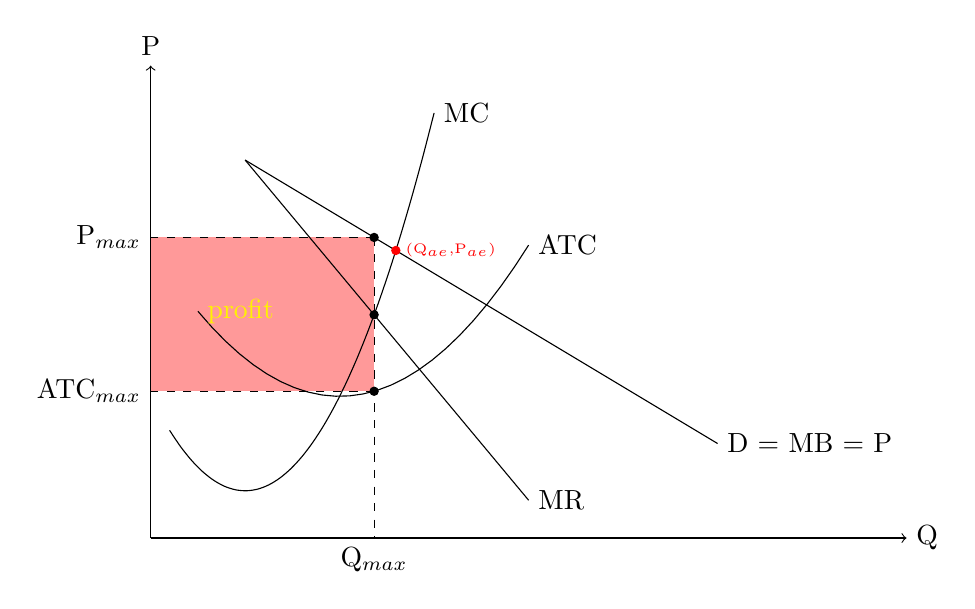
\begin{tikzpicture}[scale=1.2]
    \fill [red!40!white] (0,1.5532)--(0,3.18119)--(2.36469,3.18119)--(2.36469,1.5532);

\draw[->] (0,0)--(8,0) node[right]{Q};
\draw[->] (0,0)--(0,5) node[above]{P};

\draw[domain=0.2:3, smooth]
    plot (\x, {(\x-1)^2 + 0.5}) node[right]{MC};

\draw[domain=0.5:4]
    plot (\x, {0.4*(\x-2)^2 + 1.5}) node[right]{ATC}; 
    \draw (1,4)--(6,1) node[right]{D $=$ MB $=$ P};
    \draw (1,4)--(4,0.4) node[right]{MR};
    \node [circle,fill=black,inner sep = 1.2pt] (A1) at (2.36469,2.3625) {};
    \node [circle,fill=black,inner sep = 1.2pt] (A2) at (2.36469,3.18119) {};
    \node [circle,fill=black,inner sep = 1.2pt] (A3) at (2.36469,1.5532) {};
    \node [circle,fill=red,inner sep = 1.2pt] (A4) at (2.59473,3.04316) {};
    \draw [red](2.59473,3.04316)--(2.59473,3.04316) node[right]{\tiny (Q$_{ae}$,P$_{ae}$)};
    \draw[dashed] (2.36469,3.18119)--(2.36469,0) node[below]{Q$_{max}$};
    \draw[dashed] (2.36469,3.18119)--(0,3.18119) node[left]{P$_{max}$};
    \draw[dashed] (2.36469,1.5532)--(0,1.5532) node[left]{ATC$_{max}$};
    \draw [yellow](0.5,2.4)--(0.5,2.4) node[right]{profit};
\end{tikzpicture}
\caption{monopoly market}
\end{figure}

\textbf{allocative inefficiency:} $\Longrightarrow$ DWL (underallocation, the firm restrict the quantity $\Longrightarrow$ P $\uparrow$) 

\begin{proof}
    Since MR=MC \& MB=P \& MR $<$ P $\Longrightarrow$ MC $<$ MB (as long as the firm in monopoly maximizes profit, it will always be allocative inefficiency) 
\end{proof}

positive profit $\Longrightarrow$ \textbf{could achieve productive efficiency} (only when MC $=$ ATC$_{min}$ $=$ MR)

normal profit $\Longrightarrow$ \textbf{productive inefficiency}\\

\textbf{sources of monopoly:} 1.owner of resources or technologies 2.economies of scale \textbf{(natural monopoly)} 3.patent or copyright (authorized by government)

\textbf{Natural Monopoly: }$\Longrightarrow$ only when economies of scale $\Longrightarrow$ Q $\uparrow$ ATC $\downarrow$ and MC is always lower than ATC

\newpage

\begin{figure}[!h]
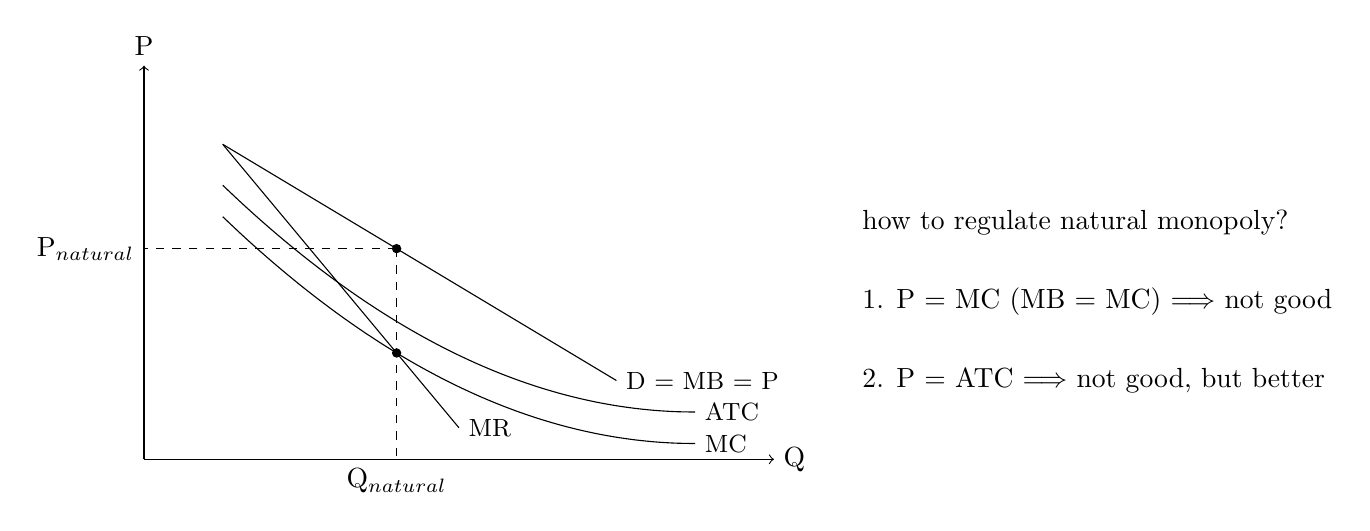
\begin{tikzpicture}
    \draw[->] (0,0)--(8,0) node[right]{Q};
    \draw[->] (0,0)--(0,5) node[above]{P};
    \draw (1,4)--(6,1) node[right]{\small D $=$ MB $=$ P};
    \draw (1,4)--(4,0.4) node[right]{\small MR};
\draw[domain=1:7, smooth]
    plot (\x, {0.08*(\x-7)^2 + 0.2}) node[right]{\small MC};
\draw[domain=1:7, smooth]
    plot (\x, {0.08*(\x-7)^2 + 0.6}) node[right]{\small ATC};
    \node [circle,fill=black,inner sep = 1.2pt] (A1) at (3.2081,1.35028) {};
    \node [circle,fill=black,inner sep = 1.2pt] (A2) at (3.2081,2.67514) {};
    \draw[dashed] (3.2081,2.67514)--(3.2081,0) node[below]{Q$_{natural}$};
    \draw[dashed] (3.2081,2.67514)--(0,2.67514) node[left]{P$_{natural}$};
    \draw (9,3)--(9,3) node[right]{how to regulate natural monopoly?};
    \draw (9,2)--(9,2) node[right]{1. P $=$ MC (MB $=$ MC) $\Longrightarrow$ not good};
    \draw (9,1)--(9,1) node[right]{2. P $=$ ATC $\Longrightarrow$ not good, but better};
\end{tikzpicture}
\end{figure}

When P $=$ MC $\Longrightarrow$ achieve the allocative efficiency $\Longrightarrow$ P $<$ ATC $\Longrightarrow$ firm earns negative profit $\Longrightarrow$ government will subsidize the firm

When P $=$ ATC $\Longrightarrow$ DWL will be smaller than when firm chases the profit maximization quantity $\Longrightarrow$ firm earns normal profit $\Longrightarrow$ firm will oppose to the policy by $\uparrow$ ATC $\Longrightarrow$ $\uparrow$ P\\


\begin{tabular}{|c|c|c|}
    \hline
    situation & profitability & efficiency \\
    \hline
    no regulation & positive profit & DWL (underallocation)\\
    \hline
    P $=$ MC & negative profit & allocative efficient\\
    \hline
    P $=$ ATC & normal profit & less DWL than no regulation\\
    \hline
\end{tabular}\\

\textbf{Price Discrimination:} same good different prices for different consumers, seller can separate consumers according to their elasticities of demand (potential arbitrage problem $\Longrightarrow$ buy lower P and sell higher P)

Assume MC is constant and FC $=$ 0 $\Longrightarrow$ MC $=$ ATC (we do not care the cost structure, but we care the pricing strategy)

\begin{figure}[!h]
    \centering
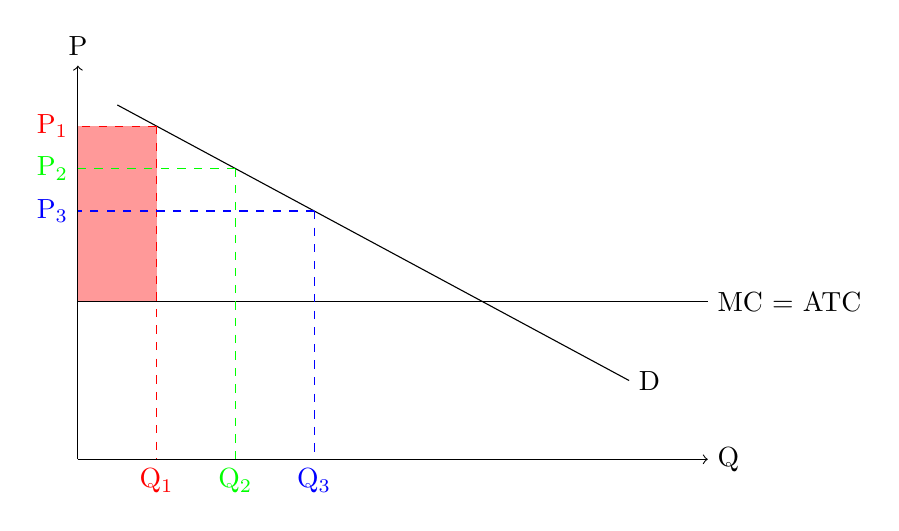
\begin{tikzpicture}
    \fill[red!40!white] (0,4.2307)--(0,2)--(1,2)--(1,4.2307);
    \draw[->] (0,0)--(8,0) node[right]{Q};
    \draw[->] (0,0)--(0,5) node[above]{P};
    \draw (0.5,4.5)--(7,1) node[right]{D};
    \draw (0,2)--(8,2) node[right]{MC $=$ ATC};
    \draw[dashed,red] (1,4.2307)--(0,4.2307) node[left]{P$_1$};
    \draw[dashed,red] (1,4.2307)--(1,0) node[below]{Q$_1$};
    \draw[dashed,green] (2,3.6922)--(0,3.6922) node[left]{P$_2$};
    \draw[dashed,green] (2,3.6922)--(2,0) node[below]{Q$_2$};
    \draw[dashed,blue] (3,3.1537)--(0,3.1537) node[left]{P$_3$};
    \draw[dashed,blue] (3,3.1537)--(3,0) node[below]{Q$_3$};
\end{tikzpicture}
\caption{price discrimination in P$_1$ P$_2$ P$_3$ (profits at different prices are important)}
\end{figure}

\textbf{Perfect Price Discrimination} (first degree price discrimination): everyone buys at the prices of maximum willingness to pay $\Longrightarrow$ no CS $\Longrightarrow$ TS $=$ PS $=$ Profit $\Longrightarrow$ no DWL (achieve allocative efficiency)

\begin{figure}[!h]
    \centering
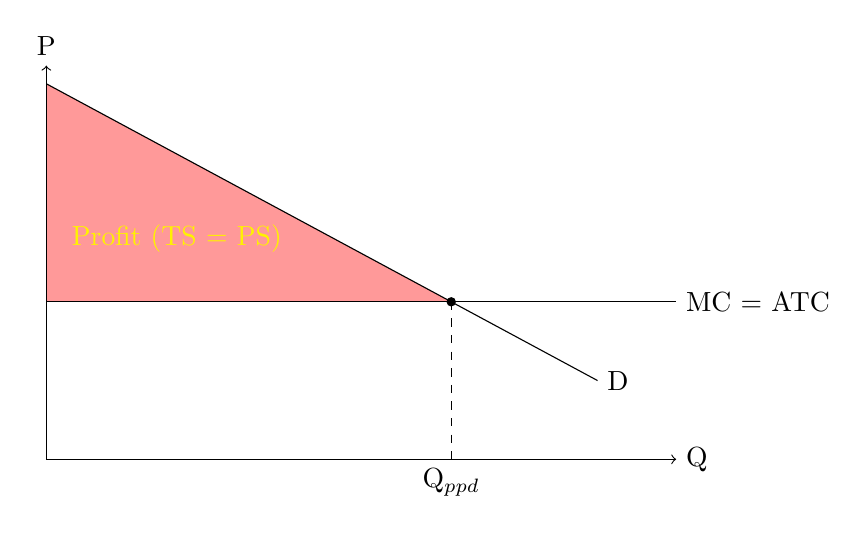
\begin{tikzpicture}
    \fill[red!40!white] (0,2)--(0,4.7692)--(5.14243,2);
    \draw[yellow] (0.2,2.8)--(0.2,2.8) node[right]{Profit (TS $=$ PS)};
    \draw[->] (0,0)--(8,0) node[right]{Q};
    \draw[->] (0,0)--(0,5) node[above]{P};
    \draw (0,4.7692)--(7,1) node[right]{D};
    \draw (0,2)--(8,2) node[right]{MC $=$ ATC};
    \node [circle,fill=black,inner sep = 1.2pt] (A1) at (5.14243,2){};
    \draw[dashed] (5.14243,2)--(5.14243,0) node[below]{Q$_{ppd}$};

\end{tikzpicture}
\caption{perfect price discrimination}
\end{figure}

\subsection{Monopolistic Competition}
\noindent

firms in the monopolistic competition market are price maker and earn normal profit (long run equilibrium)

\textbf{static assumption:} 1. lots of firms \ 2. close substitute \ 3. MR $<$ P (downward sloping demand curve)

\textbf{dynamic assumption:} easy to enter and exit (long run equilibrium)

\textbf{allocative inefficiency:} Since when MB $=$ P $>$ MC $\Longrightarrow$ never achieve allocative efficiency

\textbf{productive efficiency:} never achieve in long run, could achieve in short run (only when MC $=$ ATC$_{min}$)\\
\\
\textbf{excess capacity:} stop production when ATC is still on the decline 

\begin{figure}[!h]
    \centering
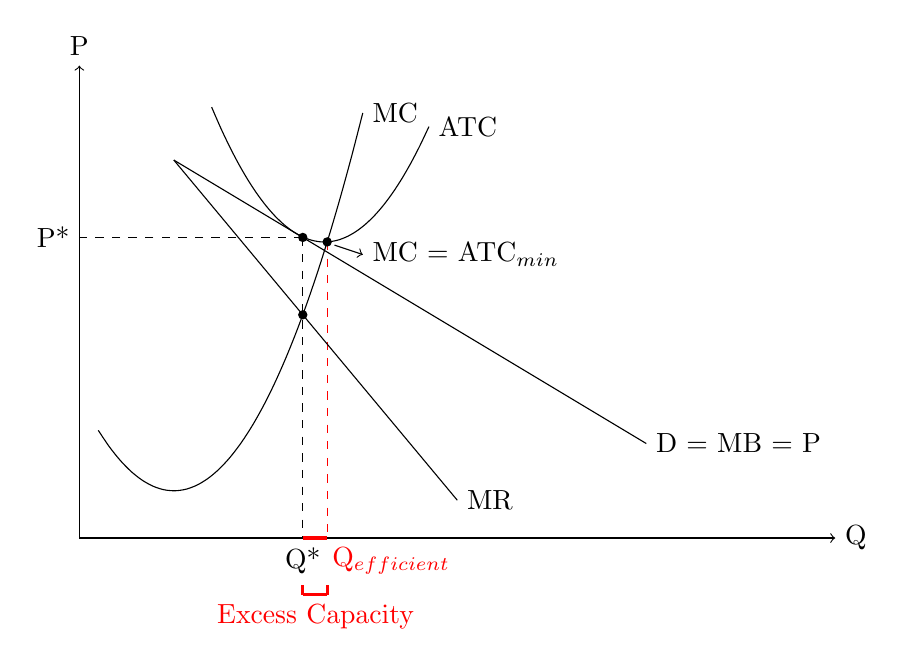
\begin{tikzpicture}[scale=1.2]

\draw[->] (0,0)--(8,0) node[right]{Q};
\draw[->] (0,0)--(0,5) node[above]{P};

\draw[domain=0.2:3, smooth]
    plot (\x, {(\x-1)^2 + 0.5}) node[right]{MC};
\draw[domain=1.4:3.7, smooth]
    plot (\x, {(\x-2.59473)^2 + 3.133}) node[right]{ATC};

    \draw[dashed,red] (2.622897,3.133793)--(2.622897,0);
    \draw [red](3.3,0)--(3.3,0) node[below]{Q$_{efficient}$};

    \draw (1,4)--(6,1) node[right]{D $=$ MB $=$ P};
    \draw (1,4)--(4,0.4) node[right]{MR};
    \node [circle,fill=black,inner sep = 1.2pt] (A1) at (2.36469,2.3625) {};
    \node [circle,fill=black,inner sep = 1.2pt] (A2) at (2.36469,3.18119) {};
    \node [circle,fill=black,inner sep = 1.2pt] (A3) at (2.622897,3.133793) {};
    \draw[->] (2.7,3.1)--(3,3) node[right]{MC $=$ ATC$_{min}$};
    \draw[dashed] (2.36469,3.18119)--(2.36469,0) node[below]{Q*};
    \draw[dashed] (2.36469,3.18119)--(0,3.18119) node[left]{P*};
    \draw[very thick,red] (2.36459,0)--(2.622897,0);
    \draw [very thick,red](2.36459,-0.6)--(2.36459,-0.5);
    \draw [very thick,red](2.622897,-0.6)--(2.622897,-0.5);
    \draw [very thick,red](2.36459,-0.6)--(2.622897,-0.6);
    \draw [red] (2.5,-0.6)--(2.5,-0.6) node[below]{Excess Capacity};
\end{tikzpicture}
\caption{long run monopolistic competition market (normal profit)}
\end{figure}

\begin{figure}[!h]
\begin{tikzpicture}
    \draw (5,5)--(8,2) node[right]{D$_1$};
    \draw (3,4)--(7,2) node[right]{D$_2$};
    \draw (10,4)--(10,4) node[right]{if more firms enter, for a specific firm's demand:};
    \draw (10,3)--(10,3) node[right]{1. decrease 2. more elastic };
\end{tikzpicture}
\end{figure}

\subsection{Oligopoly}
\noindent

firms in the oligopoly market are price maker and earn positive profit or normal profit (long run equilibrium)

\textbf{static assumption:} 1. a few firms \ 2. close substitutes or perfect substitutes \ 3. MR $<$ P (downward sloping demand curve)

\textbf{dynamic assumption:} high barrier to entry\\

Firms are \textbf{interdependent} (strategy of pricing $\rightleftarrows$ game theory)

duopoly $\longrightarrow$ when there are only 2 firms in the oligopoly market

cartel $\longrightarrow$ collaborate with each other and avoid competing with each other in order to improve their profits and dominate the market (collusion $\Longrightarrow$ monopoly)
\begin{equation}
\text{concentration ratio} = {{\Sigma (\text{Q}_1+\text{Q}_2+\text{Q}_3+\text{Q}_4)}\over \text{TQ}} \times 100\% \ \ \ \ \ \ 
\text{(Q$_1$, Q$_2$, Q$_3$, Q$_4$ $\rightarrow$ market shares of the top4 firms)}
\nonumber
\end{equation}
\subsection{Game Theory}
\noindent 

\textbf{game theory:} each party formulate optimal strategies based on the choices of others (interdependence)

\textbf{nash equilibrium:} the decision where all parties have no incentive to deviate

\textbf{dominant strategy:} strategy that brings you higher returns regardless of what your opponent chooses

\begin{figure}[!h]
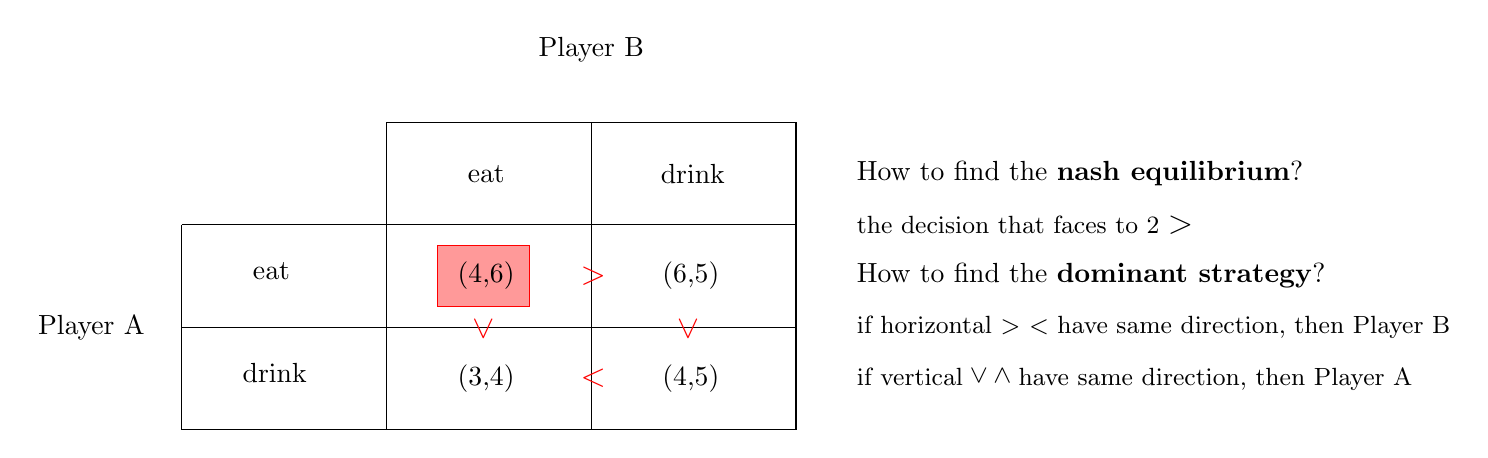
\begin{tikzpicture}[scale=1.3]
\fill [red!40!white](0.5,-0.2)--(1.4,-0.2)--(1.4,-0.8)--(0.5,-0.8);
\draw (-2,0)--(-2,-2)--(4,-2)--(4,1)--(0,1)--(0,0)--(-2,0);
\draw (0,1)--(0,-2);
\draw (-2,0)--(4,0);
\draw (-2,0)--(-2,-2);
\draw (0,1)--(4,1);
\draw (-2,-1)--(4,-1);
\draw (2,1)--(2,-2);
\draw (-1.4,-0.45)--(-1.4,-0.45) node[right]{eat};
\draw (1.25,0.5)--(1.25,0.5) node[left]{eat};
\draw (-1.5,-1.45)--(-1.5,-1.45) node[right]{drink};
\draw (3.4,0.5)--(3.4,0.5) node[left]{drink};
\draw (0.6,-0.5)--(0.6,-0.5) node[right]{(4,6)};
\draw (2.6,-0.5)--(2.6,-0.5) node[right]{(6,5)};
\draw (0.6,-1.5)--(0.6,-1.5) node[right]{(3,4)};
\draw (2.6,-1.5)--(2.6,-1.5) node[right]{(4,5)};
\draw (-3.5,-1)--(-3.5,-1) node[right]{Player A};
\draw (2,1.5)--(2,1.5) node[above]{Player B};
\draw [red](1.8,-0.5)--(1.8,-0.5) node[right]{\large $>$};
\draw [red](1.8,-1.5)--(1.8,-1.5) node[right]{\large $<$};
\draw [red] (1,-0.8)--(1,-0.8) node[below]{\large \rotatebox{90}{$<$} \quad};
\draw [red] (3,-0.8)--(3,-0.8) node[below]{\large \rotatebox{90}{$<$} \quad};
\draw [red] (0.5,-0.2)--(1.4,-0.2)--(1.4,-0.8)--(0.5,-0.8)--(0.5,-0.2);
\draw (4.5,0.5)--(4.5,0.5) node[right]{How to find the \textbf{nash equilibrium}?};
\draw (4.5,0)--(4.5,0) node[right]{\small the decision that faces to 2 \large{$>$}};
\draw (4.5,-0.5)--(4.5,-0.5) node[right]{How to find the \textbf{dominant strategy}?};
\draw (4.5,-1)--(4.5,-1) node[right]{\small if horizontal $>$ $<$ have same direction, then Player B};
\draw (4.5,-1.5)--(4.5,-1.5) node[right]{\small if vertical \rotatebox{90}{$<$} \rotatebox{90}{$>$} have same direction, then Player A};

\end{tikzpicture}
\caption{game theory example (nash equilibrium, dominant strategy)}
\end{figure}

\section{Factor Markets}
\noindent

\textcolor{red}{\textbf{\Large Input}} {\Large$\longrightarrow$ \textbf{Production} $\longrightarrow$ \textbf{Output}}

Factors of production: land, labor, capital (machine \& equipment), entrepreneurship

\subsection{Factor Demand and Factor Supply}
\noindent

\textbf{factor demand:}

\begin{figure}[!h]
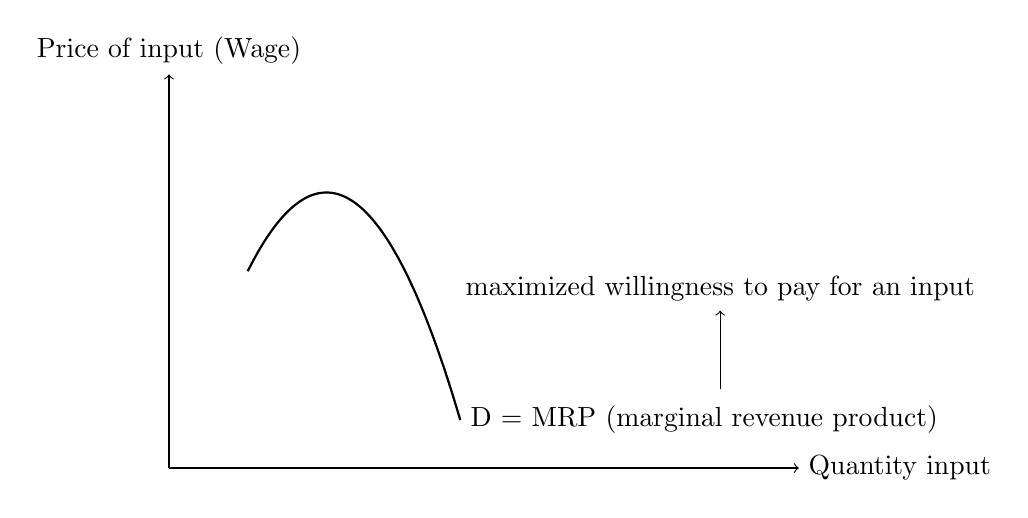
\begin{tikzpicture}
    \draw[->] (0,0)--(8,0) node[right]{Quantity input};
    \draw[->] (0,0)--(0,5) node[above]{Price of input (Wage)};
\draw[domain=1:3.7, smooth,thick]
    plot (\x, {-(\x-2)^2 + 3.5}) node[right]{D $=$ MRP (marginal revenue product)};
    \draw[->] (7,1)--(7,2) node[above]{maximized willingness to pay for an input};
\end{tikzpicture}
\caption{factor demand}
\end{figure}

{\large{MRP $=$ output price $\times$ marginal product $=$ P $\times$ MP} \ \ (MRP $\ge$ wage)}

MRP is the marginal revenue created by using one additional unit of resource

Profit maximization in factor market $\Longrightarrow$ MRP $=$ MFC (marginal factor cost)

\begin{figure}[!h]
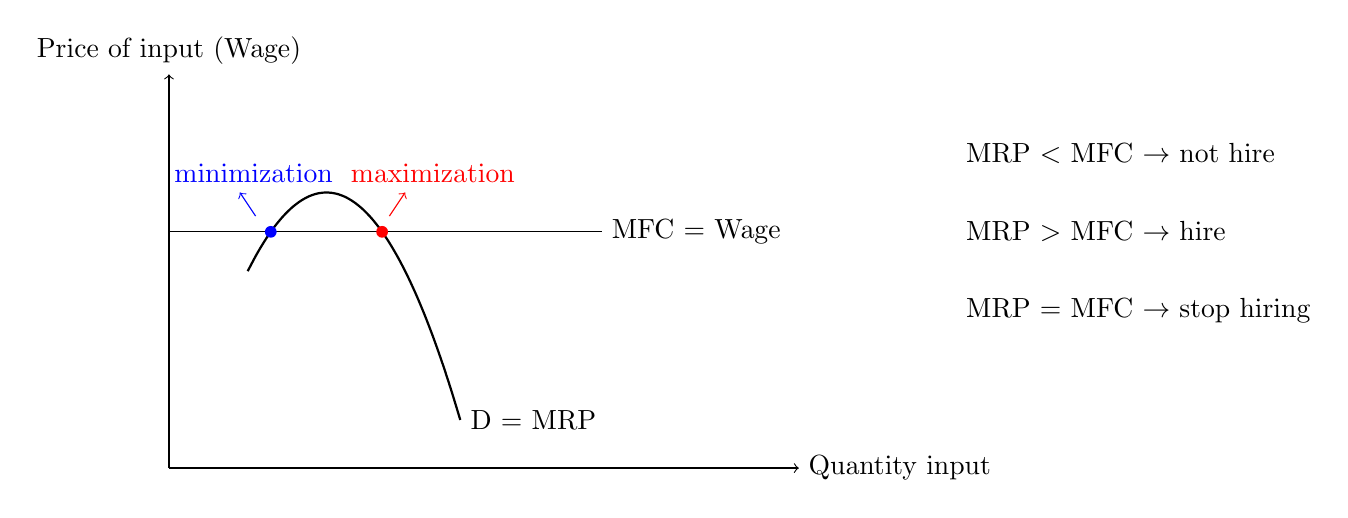
\begin{tikzpicture}
    \draw[->] (0,0)--(8,0) node[right]{Quantity input};
    \draw[->] (0,0)--(0,5) node[above]{Price of input (Wage)};
\draw[domain=1:3.7, smooth,thick]
    plot (\x, {-(\x-2)^2 + 3.5}) node[right]{D $=$ MRP};
    \draw (0,3)--(5.5,3) node[right]{MFC $=$ Wage};
    \node [circle,fill=blue,inner sep = 1.5pt] (A1) at (1.29289,3){};
    \node [circle,fill=red,inner sep = 1.5pt] (A1) at (2.70711,3){};
    \draw[red,->] (2.8,3.2)--(3,3.5) node[above]{\ \ \ \ \ \ maximization};
    \draw[blue,->] (1.1,3.2)--(0.9,3.5) node[above]{\ \ \ minimization};
    \draw (10,4)--(10,4) node[right]{MRP $<$ MFC $\rightarrow$ not hire};
    \draw (10,3)--(10,3) node[right]{MRP $>$ MFC $\rightarrow$ hire};
    \draw (10,2)--(10,2) node[right]{MRP $=$ MFC $\rightarrow$ stop hiring};
\end{tikzpicture}
\caption{profit maximization (MRP $=$ MFC)}
\end{figure}

\textbf{factor demand shifters:} 1. output price \ 2. change in MP (education \& technology)

\textbf{factor supply shifters:} 1. size of population \ 2. labor participation rate \ 3. tax and benefits policy \ 4. immigration

\textbf{least-cost rule:} A firm minimizes the cost of producing a given level of output when:

\begin{equation}
    {\text{MP}_L\over\text{P}_L} = {\text{MP}_K\over\text{P}_K} \ \ \ \ \text{where } L \longrightarrow \text{labor, } K \longrightarrow \text{capital }
    \nonumber
\end{equation}

\subsection{Perfect Competition (Factor Market)}

\begin{figure}[!h]
    \centering
\begin{tikzpicture}
    \draw [->](0,0)--(8,0) node[right]{Quantity input};
    \draw [->](0,0)--(0,5) node[above]{Wage};
    \draw [thick] (0.5,4)--(6,0.5) node[right]{D $=$ MRP};
    \draw [thick] (0.5,0.5)--(6,4) node[right]{S $=$ MFC};
    \node [circle,fill=black,inner sep = 1.5pt] (A1) at (3.25,2.25) {};
    \draw[dashed] (3.25,2.25)--(3.25,0) node[below]{Q$_e$};
    \draw[dashed] (3.25,2.25)--(0,2.25) node[left]{Wage$_e$};
\end{tikzpicture}
\caption{perfect competition factor market}
\end{figure}

\subsection{Monopsony}

\begin{figure}[!h]
    \centering
\begin{tikzpicture}
    \draw [->](0,0)--(8,0) node[right]{Quantity input};
    \draw [->](0,0)--(0,5) node[above]{Wage};
    \draw [thick] (0.5,4)--(6,0.5) node[right]{D $=$ MRP};
    \draw [thick] (0.5,0.5)--(6,4) node[right]{S};
    \draw [thick] (0.5,0.5)--(3.5,4.31818) node[right]{MFC};
    \node [circle,fill=black,inner sep = 1.5pt] (A1) at (2.333,2.833){};
    \node [circle,fill=black,inner sep = 1.5pt] (A2) at (2.333,1.667){};
    \draw[dashed] (2.333,2.833)--(2.333,0) node[below]{Q$_{max}$};
    \draw[dashed] (2.333,1.667)--(0,1.667) node[left]{Wage$_{max}$};

\end{tikzpicture}
\caption{monopsony}
\end{figure}















\newpage
\section{Market Failure}
\noindent

Sometimes the free market cannot achieve optimal allocation of resources (inefficient allocation). 

{\large market outcome $\ne$ social optimal}

\subsection{Externality}
\noindent

{\large if marginal social cost (MSC) $\ne$ marginal social benefit (MSB) $\Longrightarrow$ market failure}

\textbf{Externality:} individual's actions affect others, but this influence is not reflected in prices.

positive externality: education, vaccine | negative externality: pollution, noise\\


{\large \textbf{Positive Externality:}}

\begin{figure}[!h]
    \centering
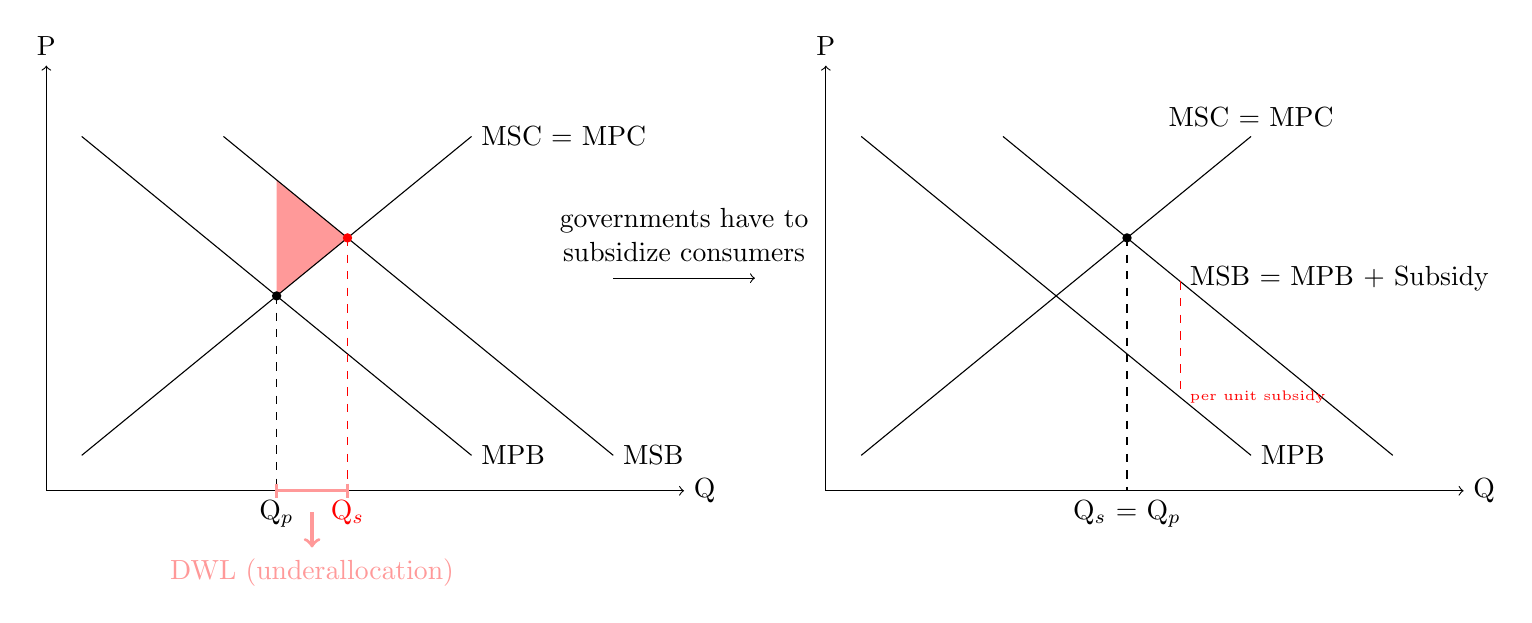
\begin{tikzpicture}[scale=0.9]
    \fill[red!40!white] (4.25,3.56818)--(3.25,2.75)--(3.25,4.38636);
    \draw[->] (0,0)--(9,0) node[right]{Q};
    \draw[->] (0,0)--(0,6) node[above]{P};
    \draw (0.5,5)--(6,0.5) node[right]{MPB};
    \draw (2.5,5)--(8,0.5) node[right]{MSB};
    \draw (0.5,0.5)--(6,5) node[right]{MSC $=$ MPC};
    \node [circle,fill=red,inner sep = 1.2pt] (A1) at (4.25,3.56818){};
    \node [circle,fill=black,inner sep = 1.2pt] (A2) at (3.25,2.75){};
    \draw[dashed,red] (4.25,3.56818)--(4.25,0) node[below]{Q$_s$};
    \draw[dashed] (3.25,2.75)--(3.25,0) node[below]{Q$_p$};
    \draw[red!40!white,very thick] (4.25,0)--(3.25,0);
    \draw[red!40!white,very thick] (4.25,0.1)--(4.25,-0.1);
    \draw[red!40!white,very thick] (3.25,0.1)--(3.25,-0.1);
    \draw[red!40!white,very thick,->] (3.75,-0.3)--(3.75,-0.8) node[below]{DWL (underallocation)};
    \draw (9,3.5)--(9,3.5) node[above]{governments have to};
    \draw (9,3.1)--(9,3.1) node[above]{subsidize consumers};
    \draw[->](8,3)--(10,3);

    \draw[->] (11,0)--(20,0) node[right]{Q};
    \draw[->] (11,0)--(11,6) node[above]{P};
    \draw (11.5,5)--(17,0.5) node[right]{MPB};
    \draw (13.5,5)--(19,0.5);
    \node [circle,fill=black,inner sep = 1.2pt] (A1) at (15.25,3.56818){};
    \draw (16,3)--(16,3) node[right]{MSB $=$ MPB + Subsidy};
    \draw (11.5,0.5)--(17,5) node[above]{MSC $=$ MPC};
    \draw[dashed] (15.25,3.56818)--(15.25,0) node[below]{Q$_s$ $=$ Q$_p$};
    \draw[red,dashed] (16,2.95455)--(16,1.31818) node[right]{\tiny per unit subsidy};
\end{tikzpicture}
\end{figure}

{\large \textbf{Negative Externality:}}

\begin{figure}[!h]
    \centering
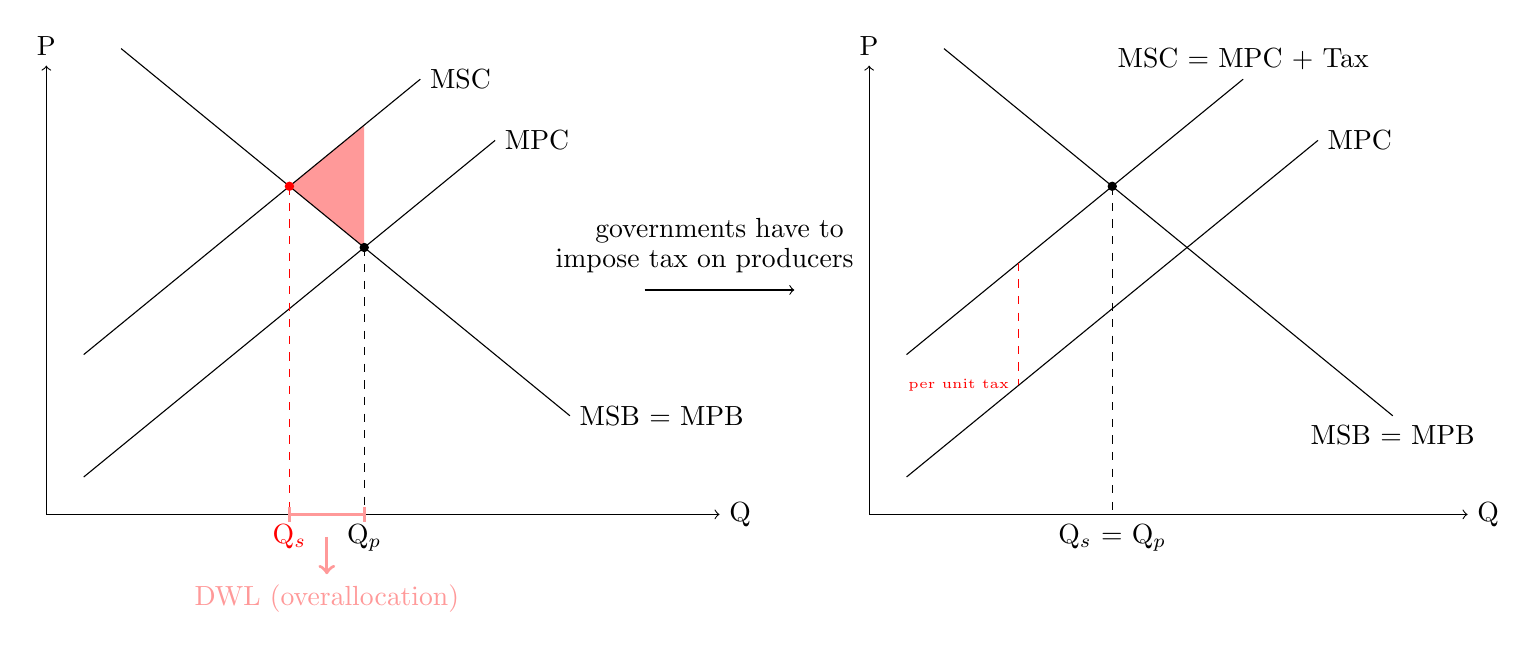
\begin{tikzpicture}[scale=0.95]
    \fill[red!40!white] (4.25,3.56818)--(4.25,5.20455)--(3.25,4.38636);
    \draw[->] (0,0)--(9,0) node[right]{Q};
    \draw[->] (0,0)--(0,6) node[above]{P};
    \draw (1,6.22727)--(7,1.31818) node[right]{MSB $=$ MPB};
    \draw (0.5,0.5)--(6,5) node[right]{MPC};
    \draw (0.5,2.13636)--(5,5.81818) node[right]{MSC};
    \node [circle,fill=black,inner sep = 1.2pt] (A1) at (4.25,3.56818){};
    \node [circle,fill=red,inner sep = 1.2pt] (A2) at (3.25,4.38636){};
    \draw[dashed] (4.25,3.56818)--(4.25,0) node[below]{Q$_p$};
    \draw[dashed,red] (3.25,4.38636)--(3.25,0) node[below]{Q$_s$};
    \draw[red!40!white,very thick] (4.25,0)--(3.25,0);
    \draw[red!40!white,very thick] (4.25,0.1)--(4.25,-0.1);
    \draw[red!40!white,very thick] (3.25,0.1)--(3.25,-0.1);
    \draw[red!40!white,very thick,->] (3.75,-0.3)--(3.75,-0.8) node[below]{DWL (overallocation)};

    \draw (9,3.5)--(9,3.5) node[above]{governments have to};
    \draw (8.8,3.1)--(8.8,3.1) node[above]{impose tax on producers};
    \draw[->](8,3)--(10,3);

    \draw[->] (11,0)--(19,0) node[right]{Q};
    \draw[->] (11,0)--(11,6) node[above]{P};
    \draw (12,6.22727)--(18,1.31818) node[below]{MSB $=$ MPB};
    \draw (11.5,0.5)--(17,5) node[right]{MPC};
    \draw (11.5,2.13636)--(16,5.81818) node[above]{MSC $=$ MPC + Tax};
    \node [circle,fill=black,inner sep = 1.2pt] (A2) at (14.25,4.38636){};
    \draw[dashed] (14.25,4.38636)--(14.25,0) node[below]{Q$_s$ $=$ Q$_p$};
    \draw[red,dashed] (13,3.36364)--(13,1.72727) node[left]{\tiny per unit tax};

\end{tikzpicture}
\end{figure}

solution to negative externality: 1. corrective tax \ 2. direct regulation \ 3. privatization

solution to positive externality: 1. corrective subsidy

\textbf{Coase theorem:} private policy to solve negative externality (negotiation among private parties, problem: probably transaction cost) 

\subsection{Excludability \& Rivalry}

\begin{figure}[!h]
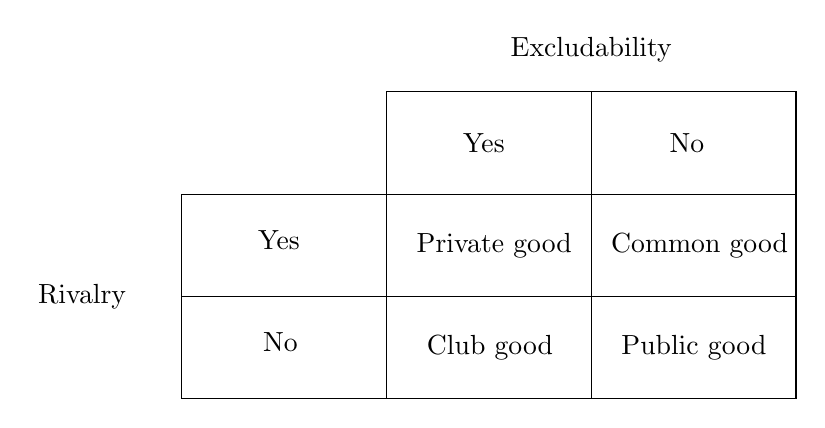
\begin{tikzpicture}[scale=1.3]
\draw (-2,0)--(-2,-2)--(4,-2)--(4,1)--(0,1)--(0,0)--(-2,0);
\draw (0,1)--(0,-2);
\draw (-2,0)--(4,0);
\draw (-2,0)--(-2,-2);
\draw (0,1)--(4,1);
\draw (-2,-1)--(4,-1);
\draw (2,1)--(2,-2);
\draw (-1.35,-0.45)--(-1.35,-0.45) node[right]{Yes};
\draw (1.25,0.5)--(1.25,0.5) node[left]{Yes};
\draw (-1.3,-1.45)--(-1.3,-1.45) node[right]{No};
\draw (3.2,0.5)--(3.2,0.5) node[left]{No};
\draw (0.2,-0.5)--(0.2,-0.5) node[right]{Private good};
\draw (2.1,-0.5)--(2.1,-0.5) node[right]{Common good};
\draw (0.3,-1.5)--(0.3,-1.5) node[right]{Club good};
\draw (2.2,-1.5)--(2.2,-1.5) node[right]{Public good};
\draw (-3.5,-1)--(-3.5,-1) node[right]{Rivalry};
\draw (2,1.2)--(2,1.2) node[above]{Excludability};
\end{tikzpicture}
\end{figure}


\textbf{rivalry:} one person’s consumption of a good reduces the amount available for others

non-rival $\longrightarrow$ MC $=$ 0

\textbf{excludability:} people can be prevented from using a good if they do not pay for it

non-excludable $\longrightarrow$ P $=$ 0\\

\begin{tabular}{|c|c|c|c|c|}
    \hline
    type of goods & rival? & excludable? & examples & problem\\
    \hline
    private goods & \ding{51} & \ding{51} & car, food & no\\
    \hline
    public goods & \ding{55} & \ding{55} & national defense & free rider problem\\
    \hline
    common goods & \ding{51} & \ding{55} & fish & overusing\\
    \hline
    club goods & \ding{55} & \ding{51} & toll highway, membership & congestion\\
    \hline
\end{tabular}\\

\textbf{common goods} (fishing) $\longrightarrow$ tragedy of commons (overusing problem) $\longrightarrow$ negative externality

$\because$ amount of fish is limited (rival), but anyone can go fishing (non-excludable) $\longrightarrow$ overusing $\longrightarrow$ resource depleted 

\textbf{public goods} $\longrightarrow$ free rider problem $\longrightarrow$ positive externality

$\because$ unable to prevent others from using it $\longrightarrow$ no one wants to pay $\longrightarrow$ market supply insufficient 

\newpage
\subsection{Inequality}
\noindent
\\
\begin{tabular}{|c|c|c|c|}
    \hline
    type of tax & definition & example & influence\\
    \hline
    progressive tax & poor pay a smaller proportion of their income than the rich & income tax & income inequality $\downarrow$\\
    \hline
    regressive tax & poor pay a larger proportion of their income than the rich & sales tax & income inequality $\uparrow$\\
    \hline
    proportional tax & same proportion for everyone & - & -\\
    \hline
\end{tabular}\\

How to reduce the income inequality? 1. progressive tax \ 2. education \\

\textbf{\large Lorenz Curve}

\begin{figure}[!h]
    \centering
\begin{tikzpicture}
    \draw[very thick] (4,3)--(4,3) node[right]{\Large A};
    \draw[very thick] (7,3)--(7,3) node[right]{\Large B};
    \draw[dotted,thick] (5,2.5)--(5,0);
    \draw[dotted,thick] (5,2.5)--(10,2.5);
    \draw[->,thick] (0,0)--(10,0);
    \draw[->,thick] (10,0)--(10,10);
    \draw (1,0.1)--(1,0) node[below]{10};
    \draw (2,0.1)--(2,0) node[below]{20};
    \draw (3,0.1)--(3,0) node[below]{30};
    \draw (4,0.1)--(4,0) node[below]{40};
    \draw (5,0.1)--(5,0) node[below]{50};
    \draw (6,0.1)--(6,0) node[below]{60};
    \draw (7,0.1)--(7,0) node[below]{70};
    \draw (8,0.1)--(8,0) node[below]{80};
    \draw (9,0.1)--(9,0) node[below]{90};
    \draw (10,0.1)--(10,0) node[below]{100};
    \draw (9.9,1)--(10,1) node[right]{10};
    \draw (9.9,2)--(10,2) node[right]{20};
    \draw (9.9,3)--(10,3) node[right]{30};
    \draw (9.9,4)--(10,4) node[right]{40};
    \draw (9.9,5)--(10,5) node[right]{50};
    \draw (9.9,6)--(10,6) node[right]{60};
    \draw (9.9,7)--(10,7) node[right]{70};
    \draw (9.9,8)--(10,8) node[right]{80};
    \draw (9.9,9)--(10,9) node[right]{90};
    \draw (9.9,10)--(10,10) node[right]{100};


    \draw [red!80!white](6,5)--(6,5) node[right]{Lorenz curve};
    \draw (5,-0.5)--(5,-0.5) node[below]{cumulative population (\%)};
    \draw (11,5)--(11,5) node[right]{cumulative share of wealth (\%)};
    \draw (0,0)--(10,10);
    \draw (2.5,5.5)--(2.5,5.5) node[right]{line of equality};
\draw[domain=0:10, smooth,red!40!white]
    plot (\x, {0.1*(\x)^2});
\end{tikzpicture}
\caption{e.g. 50\% population (poorest - richest) $\Longrightarrow$ 25\% wealth}
\end{figure}

\textbf{Gini coefficient:} 

\begin{equation}
    \text{Gini coefficient} = {A\over {A+B}}
    \nonumber
\end{equation}

when Gini coefficient = 0 $\Longrightarrow$ perfect equality

when Gini coefficient = 1 $\Longrightarrow$ maximal inequality






\end{document}